\documentclass[%
 reprint,
%superscriptaddress,
%groupedaddress,
%unsortedaddress,
%runinaddress,
%frontmatterverbose, 
%preprint,
%showpacs,preprintnumbers,
nofootinbib,
%nobibnotes,
%bibnotes,
 amsmath,amssymb,
 aps,
pra,
%prb,
%rmp,
%prstab,
%prstper,
floatfix,
]{revtex4-2}

\usepackage{braket}
%\usepackage{subcaption}
\usepackage{dsfont}
%\usepackage{hyperref}
\usepackage{graphicx}% Include figure files
\graphicspath{{images/}}
\usepackage{dcolumn}% Align table columns on decimal point
\usepackage{bm}% bold math
\usepackage{mathtools}
\usepackage[thinc]{esdiff}
\usepackage{textcomp}
\usepackage{subfigure}
%\usepackage{xcolor}
\usepackage[dvipsnames]{xcolor}
\usepackage{appendix}
\usepackage{tcolorbox}
\usepackage{multirow}
\usepackage{tikz}




\newtheorem{theorem}{Theorem}

\newtheorem{definition}{Definition}

%\def\bibsection{\section*{References}}        % Position reference section correctly

\newcommand{\me}[3]{ \langle #1|#2|#3\rangle }
\newcommand{\ad}[1]{{\bf \color{orange}{[AD] #1}}}
\newcommand{\tikzcircle}[2][red,fill=red]{\tikz[baseline=-0.5ex]\draw[#1,radius=#2] (0,0) circle ;}%
%%%%% Document %%%%%    
\begin{document}

\title{Quantum Optimization for Graph Coloring Problem Using Rydberg-Qutrit Arrays with Successive Local Driving Technique} 
\date{Submitted: \today{}}
\author{Toonyawat Angkhanawin}
\affiliation{\normalfont \textit{Joint Quantum Centre (Durham-Newcastle), Department of Physics, Durham University, South Road, Durham, DH1 3LE, United Kingdom}}
\author{Aydin Deger}
\affiliation{Department of Physics and Astronomy, University College London, London WC1E 6BT, United Kingdom}
\author{C. Stuart Adams}
\affiliation{\normalfont \textit{Joint Quantum Centre (Durham-Newcastle), Department of Physics, Durham University, South Road, Durham, DH1 3LE, United Kingdom}}


\begin{abstract}
Rydberg atoms have shown remarkably high potential as a candidate for a quantum simulator and quantum computing platform. One of the very famous application that could highly benefit from Rydberg atoms is quantum optimization. In this work, we design new architectures for quantum optimization using one-dimensional arrays of Rydberg-atom qutrits where each atom is coherently coupled to two different Rydberg states, giving rise to three types of long-range van de Waals interactions. Each interaction contributes to different penalized terms in Hamiltonian cost function which plays very crucial roles in the optimization processes. In this work, we are focusing on solving the so-called graph coloring problem (GCP), which is known as NP-hard in computer science. It has been found that solutions of GCPs could be encoded in ground states of this interacting Rydberg-qutrit Hamiltonian, and such solutions can be delivered by quantum optimization schemes we develop, which are implemented via quantum annealing algorithms based on adiabatic quantum computation. One of the highlighted features of this optimization scheme is the ability to perform two-laser detuning sweeping with different orders in time fashion. This could alter adiabatic trajectory paths and drive annealing states into different low energy sub-spaces, paving us a way to use such quantum optimizers to solve the optimization with associated constraints which is hard in classical optimization.
\end{abstract}

\maketitle
%\thispagestyle{plain} % produces page number for front page

\section{Introduction}
The collective behaviours in many-body quantum systems have been a very active field of research in quantum simulation and condensed matter physics. The systems with Rydberg atoms is one of very promising platforms of quantum simulation for such many-body quantum systems, Many researches have prove their advantages over trapped ion- and superconducting-based quantum simulations in the aspects of scalability and controllability. By the advent of advanced optical-device technologies such as optical tweezers and microwave lasers, the researchers are able to accurately control an individual atom and couple a Rydberg atom with distinct Rydberg states, therefore finely tune their interaction. To study quantum many-body phenomena in some nontrivial regimes, e.g., thermodynamic limit, one has to increase the number of interacting atoms, which means growing the dimension of Hilbert space and make computational cost exponentially grow with the system size. Notably, to enhance the complexity of quantum many-body systems, enlarging the Hilbert space with computational cost growing slower than exponential rate with the system size remains one of the most challenging tasks and is therefore one of the main motive for this work.

In this work, instead of expanding Hilbert space by growing system size, i.e.,the number of atoms, we make dimension of an individual atom bigger than "qubit" but "qudit", i.e. $d>2$. In this work, we particularly interest in case where $d=3$. Generally speaking, on the case study a one-dimensional Rydberg array with each atom behaving as a "qutrit" not "qubit". In such systems, each Rydberg atom is excited homogeneously from the same ground state to two different Rydberg states, and the complexity arises from complex interactions between Rydberg atoms. As each atom being excited to two different Rydberg states gives rise to various species of short-range dipole-dipole interaction with $V_{ij} = C_3/r^3_{ij}$  and long-range Van de Waals interaction with $V_{ij} = C_6/r^6_{ij}$ between atom $\text{i}^{\text{th}}$ and atom $\text{j}^{\text{th}}$ \cite{Saffman2010QuantumAtoms}. It is of interest to understand the properties of the ground states of such systems and explore many-body phenomena that could arise from within. In previous works, we have studied the same system with each Rydberg atom behaving as a qubit composed of Rydberg and ground states. It has been shown that the ground states of such many-body Rydberg Hamiltonians exhibit certain spontaneously broken symmetries, i.e., broken $\mathbf{Z_2}$ symmetry by two-site translation, broken $\mathbf{Z_3}$ symmetry by three-site translation and broken $\mathbf{Z_4}$ symmetry by four-site translation, depending on chosen Rabi frequency and detuning terms in the Hamiltonian \cite{Bernien2017ProbingSimulator,Keesling2019QuantumSimulator}. 

\section{Theoretical background}

\subsection{Array of interacting Rydberg-atom qutrits}

\emph{Interaction between Rydberg-atom qutrits.}--- We consider a one-dimensional array of Rydberg-atom qutrits trapped in optical tweezers as shown in Fig.\ref{fig:many-qutrit}. Each atom is coherently coupled to two different highly excited, long-lived Rydberg states, i.e., $\ket{r_1}$ and $\ket{r_2}$, giving rise to different species of dipole-dipole interactions, which in general can be categorized into dipole resonant (short-range) interaction scaling with $C_3/r^3$ and van de Waals (long-range) interaction scaling with $C_6/r^6$. Here, $C_3$ and $C_6$ are respectively the energy shift factors defined by first- and second- order perturbation terms \cite{Saffman2010QuantumAtoms}. However, in this case the atom pairs of the same Rydberg excited state, i.e., $\ket{r_1r_1}$ and $\ket{r_2r_2}$, effectively yields vanishing first-order perturbation terms due to the same parity of the Rydberg states leading to zero dipole matrix elements, i.e., $C^{(1)}_3 \propto \bra{r_1}e\boldsymbol{r}\ket{r_1}^2 = 0$ and $C^{(2)}_3 \propto \bra{r_2}e\boldsymbol{r}\ket{r_2}^2 = 0$, resulting in only second-order perturbation terms ($C^{(1)}_6 \neq 0$ and $C^{(2)}_6 \neq 0$) that contribute to the energy shift of such pair states. In contrast, for the atom pair of different Rydberg excited state, i.e., $\ket{r_1r_2}$, the energy shift is in general dominated by the first order perturbation terms \cite{Saffman2010QuantumAtoms,Browaeys2020Many-bodyAtoms}. However, the first-order perturbation terms can be suppressed provided that the Rydberg states $\ket{r_1}$ and $\ket{r_2}$ are chosen to have the same parity which again vanish the dipole matrix element in first-order perturbation term, i.e., $C^{(12)}_3 \propto \bra{r_1}e\boldsymbol{r}\ket{r_2}^2 = 0$, and leave the energy shift of such pair state only contributed from the second-order perturbation $C^{(12)}_6 \neq 0$. The details of all interactions within this array of Rydberg-atom qutrits has been illustrated as Fig.\ref{fig:many-qutrit}. Such a system is the main research object considered throughout all the work here in this paper. 
\begin{figure}[ht!]
    \centering
    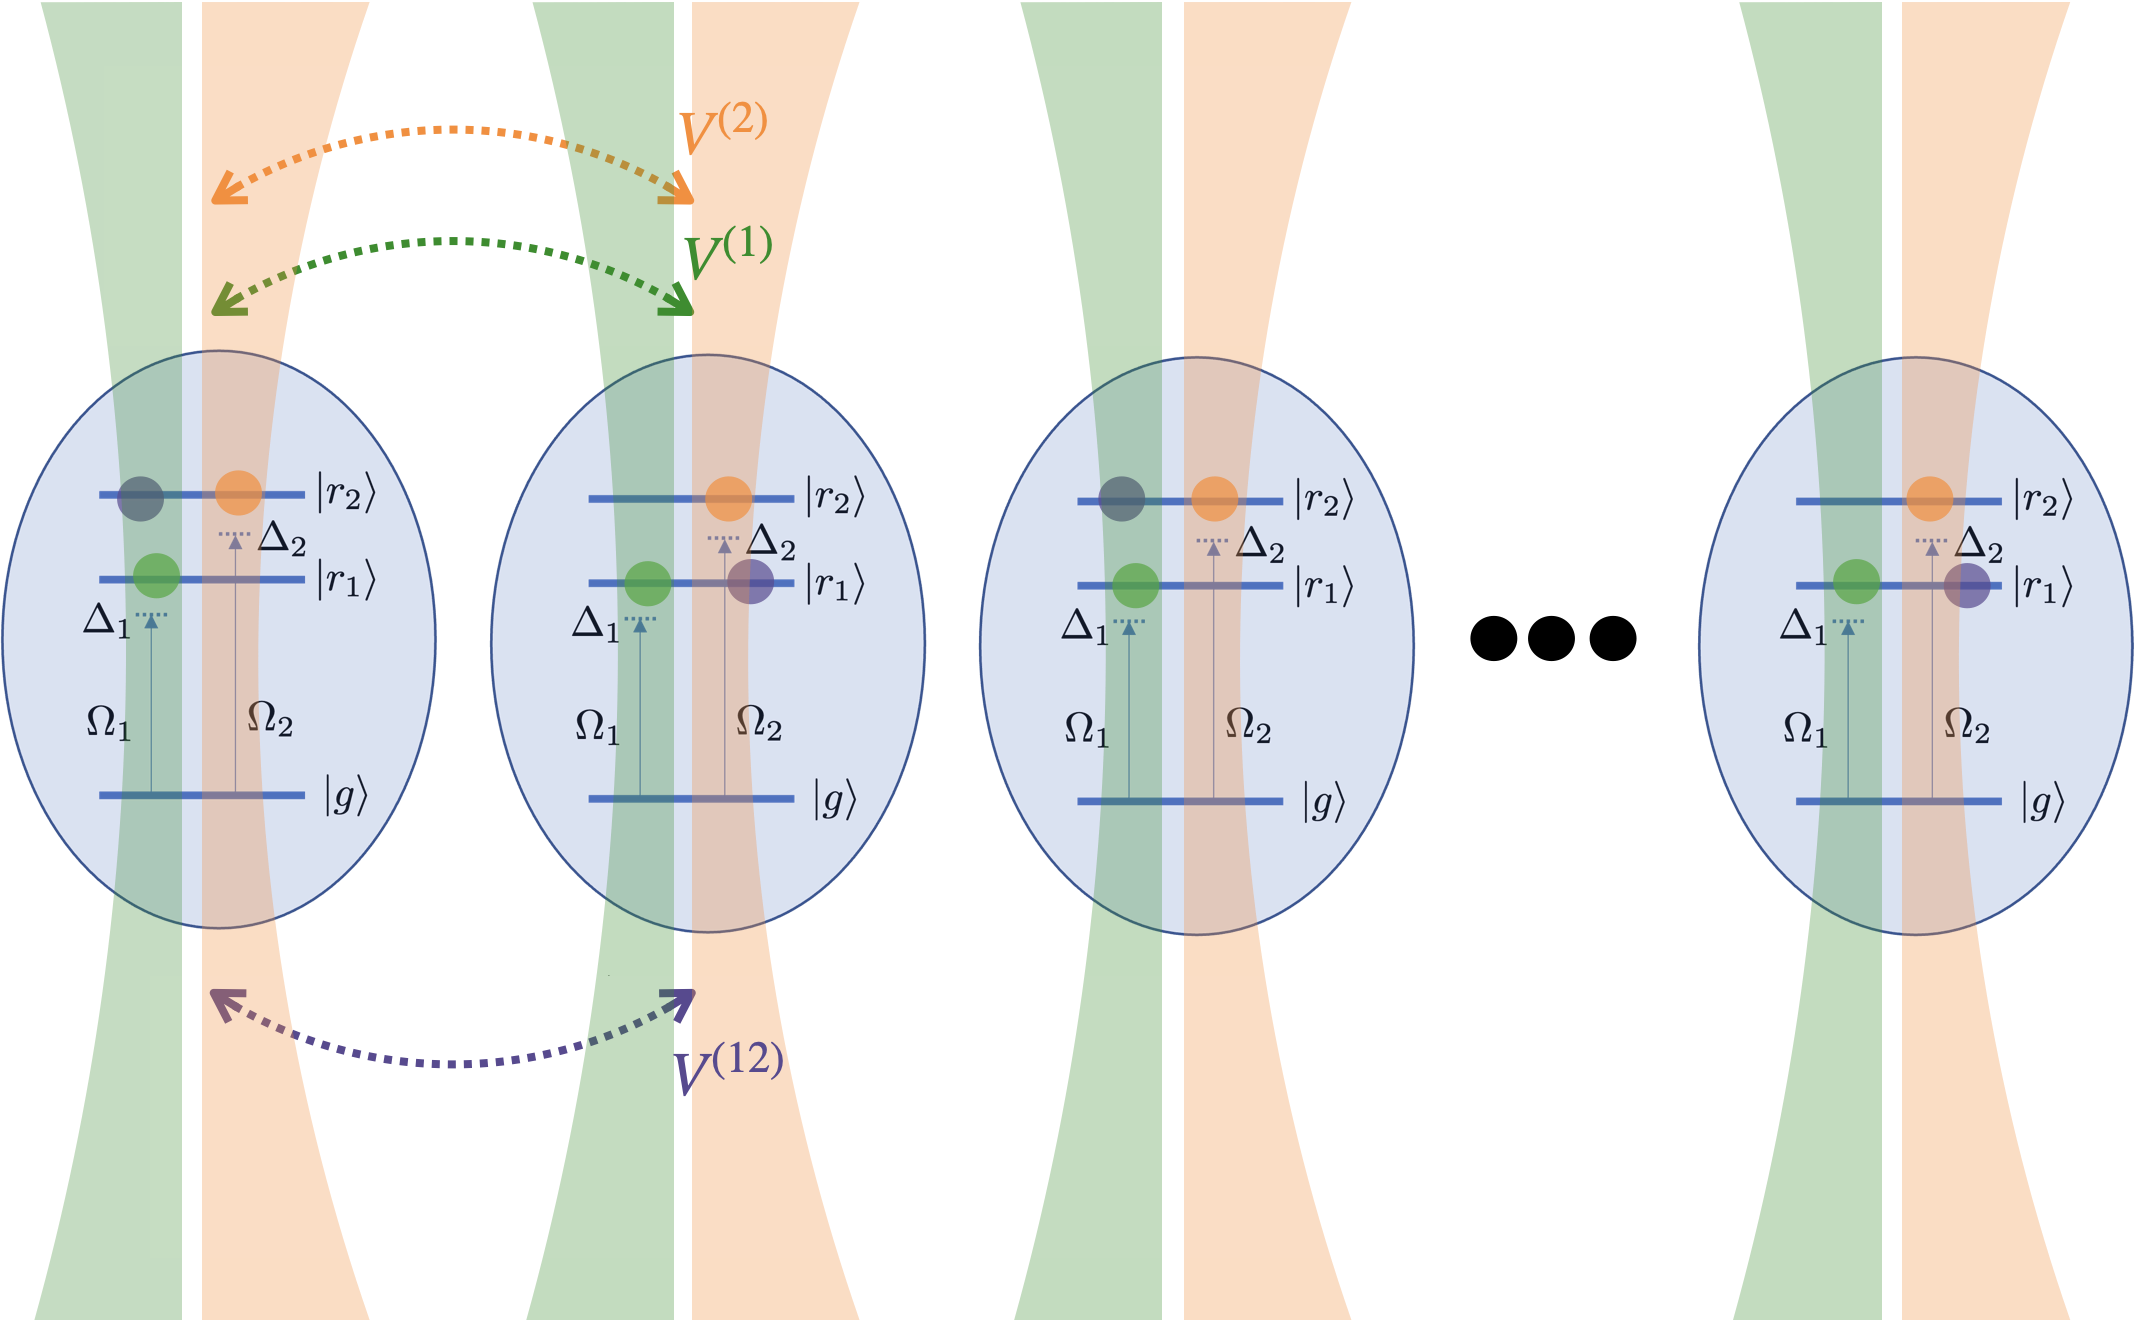
\includegraphics[width=7.8cm]{picture/many-qutrit.png}
    \caption{\textbf{Array of interacting Rydberg-atom qutrits}. The system of 1D chain of Rydberg-atom qutrits in which atomic ground states $\ket{g}$ are coherently coupled to the Rydberg states $\ket{r_1}$ and $\ket{r_2}$ by the Rabi frequencies $\Omega_1$ (green laser), $\Omega_2$ (orange laser) and the detunings $\Delta_1$ and $\Delta_2$, respectively. There are 3 types of van de Waals interactions as in following scenarios: 1.) energy shift $\propto C^{(1)}_6$ when neighbouring atoms are both excited to $\ket{r_1}$ (green circle). 2.) energy shift $\propto C^{(2)}_6$ when neighbouring atoms are both excited to $\ket{r_2}$ (orange circle). 3.) energy shift $\propto C^{(12)}_6$ when neighbouring atoms are excited to $\ket{r_1}$ and $\ket{r_2}$ (purple arrow). Since the Rydberg states $\ket{r_1}$ and $\ket{r_2}$ are chosen to have the same parity which leads to zero dipole matrix element, resulting in the suppression of resonant dipole interaction $C^{(12)}_3 = 0$. }
    \label{fig:many-qutrit}
\end{figure}

\emph{Rydberg-atom qutrit Hamiltonian.}--- As shown in Fig.\ref{fig:many-qutrit}, there is competition between 3 types of van de Waals interactions, i.e., $V^{(1)}$, $V^{(2)}$ and $V^{(12)}$, and each interaction effectively yields different Rydberg blockade mechanisms. The dynamics of such a system is governed by the Hamiltonian 

\begin{align}\label{eq:H_ryd}
H_{\textit{\rm Ryd}} &= \sum_{i} \left[ (\frac{\Omega_1}{2}\sigma^{(i)}_1 - \Delta_1 n^{(i)}_1 ) + (\frac{\Omega_2} {2}\sigma^{(i)}_2 - \Delta_2 n^{(i)}_2 ) \right] \nonumber \\ 
&+ \sum_{i<j} V^{(1)}(|\boldsymbol{r}_i - \boldsymbol{r}_j|) n^{(i)}_1 n^{(j)}_1  \nonumber \\ 
&+ \sum_{i<j} V^{(2)}(|\boldsymbol{r}_i - \boldsymbol{r}_j|) n^{(i)}_2 n^{(j)}_2 \\
&+ \sum_{i<j} V^{(12)}(|\boldsymbol{r}_i - \boldsymbol{r}_j|) n^{(i)}_1 n^{(j)}_2 \nonumber
\end{align}
where $\Omega_1$ and $\Omega_2$ are the (homogeneous) Rabi frequencies for the first and second laser driving which excite the atoms to the Rydberg states $\ket{r_1}$ and $\ket{r_2}$, respectively, $\Delta_1$ and $\Delta_2$ are the detunings for the corresponding drivings, $\sigma^{(i)}_1 = \ket{g}_i\bra{r_1} + \ket{r_1}_i \bra{g}$ and $\sigma^{(i)}_2 = \ket{g}_i\bra{r_2} + \ket{r_2}_i \bra{g}$ are analogously similar to Pauli $\sigma_x$ but for $\ket{g}$ to $\ket{r_1}$ and $\ket{g}$ to $\ket{r_2}$, respectively,  $n^{(i)}_1 = \ket{r_1}_i \bra{r_1}$ and $n^{(i)}_2 = \ket{r_2}_i \bra{r_2}$ are the projectors onto the Rydberg states $\ket{r_1}$ and $\ket{r_2}$ of atom $i^{\text{th}}$, and the 3 types of van de Waals interaction $V^{(1)}(x) = C^{(1)}_6/x^6$, $V^{(2)}(x) = C^{(2)}_6/x^6$, $V^{(12)}(x) = C^{(12)}_6/x^6$. \\

\emph{Rydberg blockade mechanisms.}--- We consider the case of homogeneous laser driving and the regime where $V^{(1)},V^{(2)},V^{(12)} > \Delta_1=\Delta_2 =\Delta > \Omega_1=\Omega_2=\Omega > 0$ The terms $\Delta_1$ and $\Delta_2$ in the Hamiltonian energetically favors each atom to be in both Rydberg states $\ket{r_1}$ and $\ket{r_2}$, while the terms $V^{(1)}$, $V^{(2)}$ and $V^{(12)}$ penalize the inclusion of atoms in the Rydberg states $\ket{r_1}$ and $\ket{r_2}$ in three different scenarios as the following (see Fig.\ref{fig:blockade}): (1) The atom $i$ and atom $j$ being simultaneously excited in $\ket{r_1}$ within certain distance $r_{ij}=|\boldsymbol{r}_i-\boldsymbol{r_j}|$ penalize the system with energy $V^{(1)}(r_{ij})$, and the simultaneous excitation in $\ket{r_1}$ is energetically prohibited when $V^{(1)}(r_{ij})>\Omega$, which happens within the characteristic distance called \emph{blockade radius} $R^{(1)}_b$, where $V^{(1)}(R^{(1)}_b)=\Omega$ (Fig.\ref{fig:blockade}(a)). (2) The atom $i$ and atom $j$ being simultaneously excited in $\ket{r_2}$ within certain distance $r_{ij}$ penalize the system with energy $V^{(2)}(r_{ij})$, and the simultaneous excitation in $\ket{r_2}$ is energetically prohibited when $V^{(2)}(r_{ij})>\Omega$, which happens within the characteristic distance $R^{(2)}_b$, where $V^{(2)}(R^{(2)}_b)=\Omega$ (Fig.\ref{fig:blockade}(b)). (3) The atom $i$ and atom $j$ being simultaneously excited in $\ket{r_1}$ and $\ket{r_2}$ within certain distance $r_{ij}$ penalize the system with energy $V^{(12)}(r_{ij})$, and the simultaneous excitation in $\ket{r_1}$ and $\ket{r_2}$ is energetically prohibited when $V^{(12)}(r_{ij})>\Omega$, which happens within the characteristic distance $R^{(12)}_b$, where $V^{(12)}(R^{(12)}_b)=\Omega$ (Fig.\ref{fig:blockade}(c)).
\begin{figure}[ht!]
    \centering
    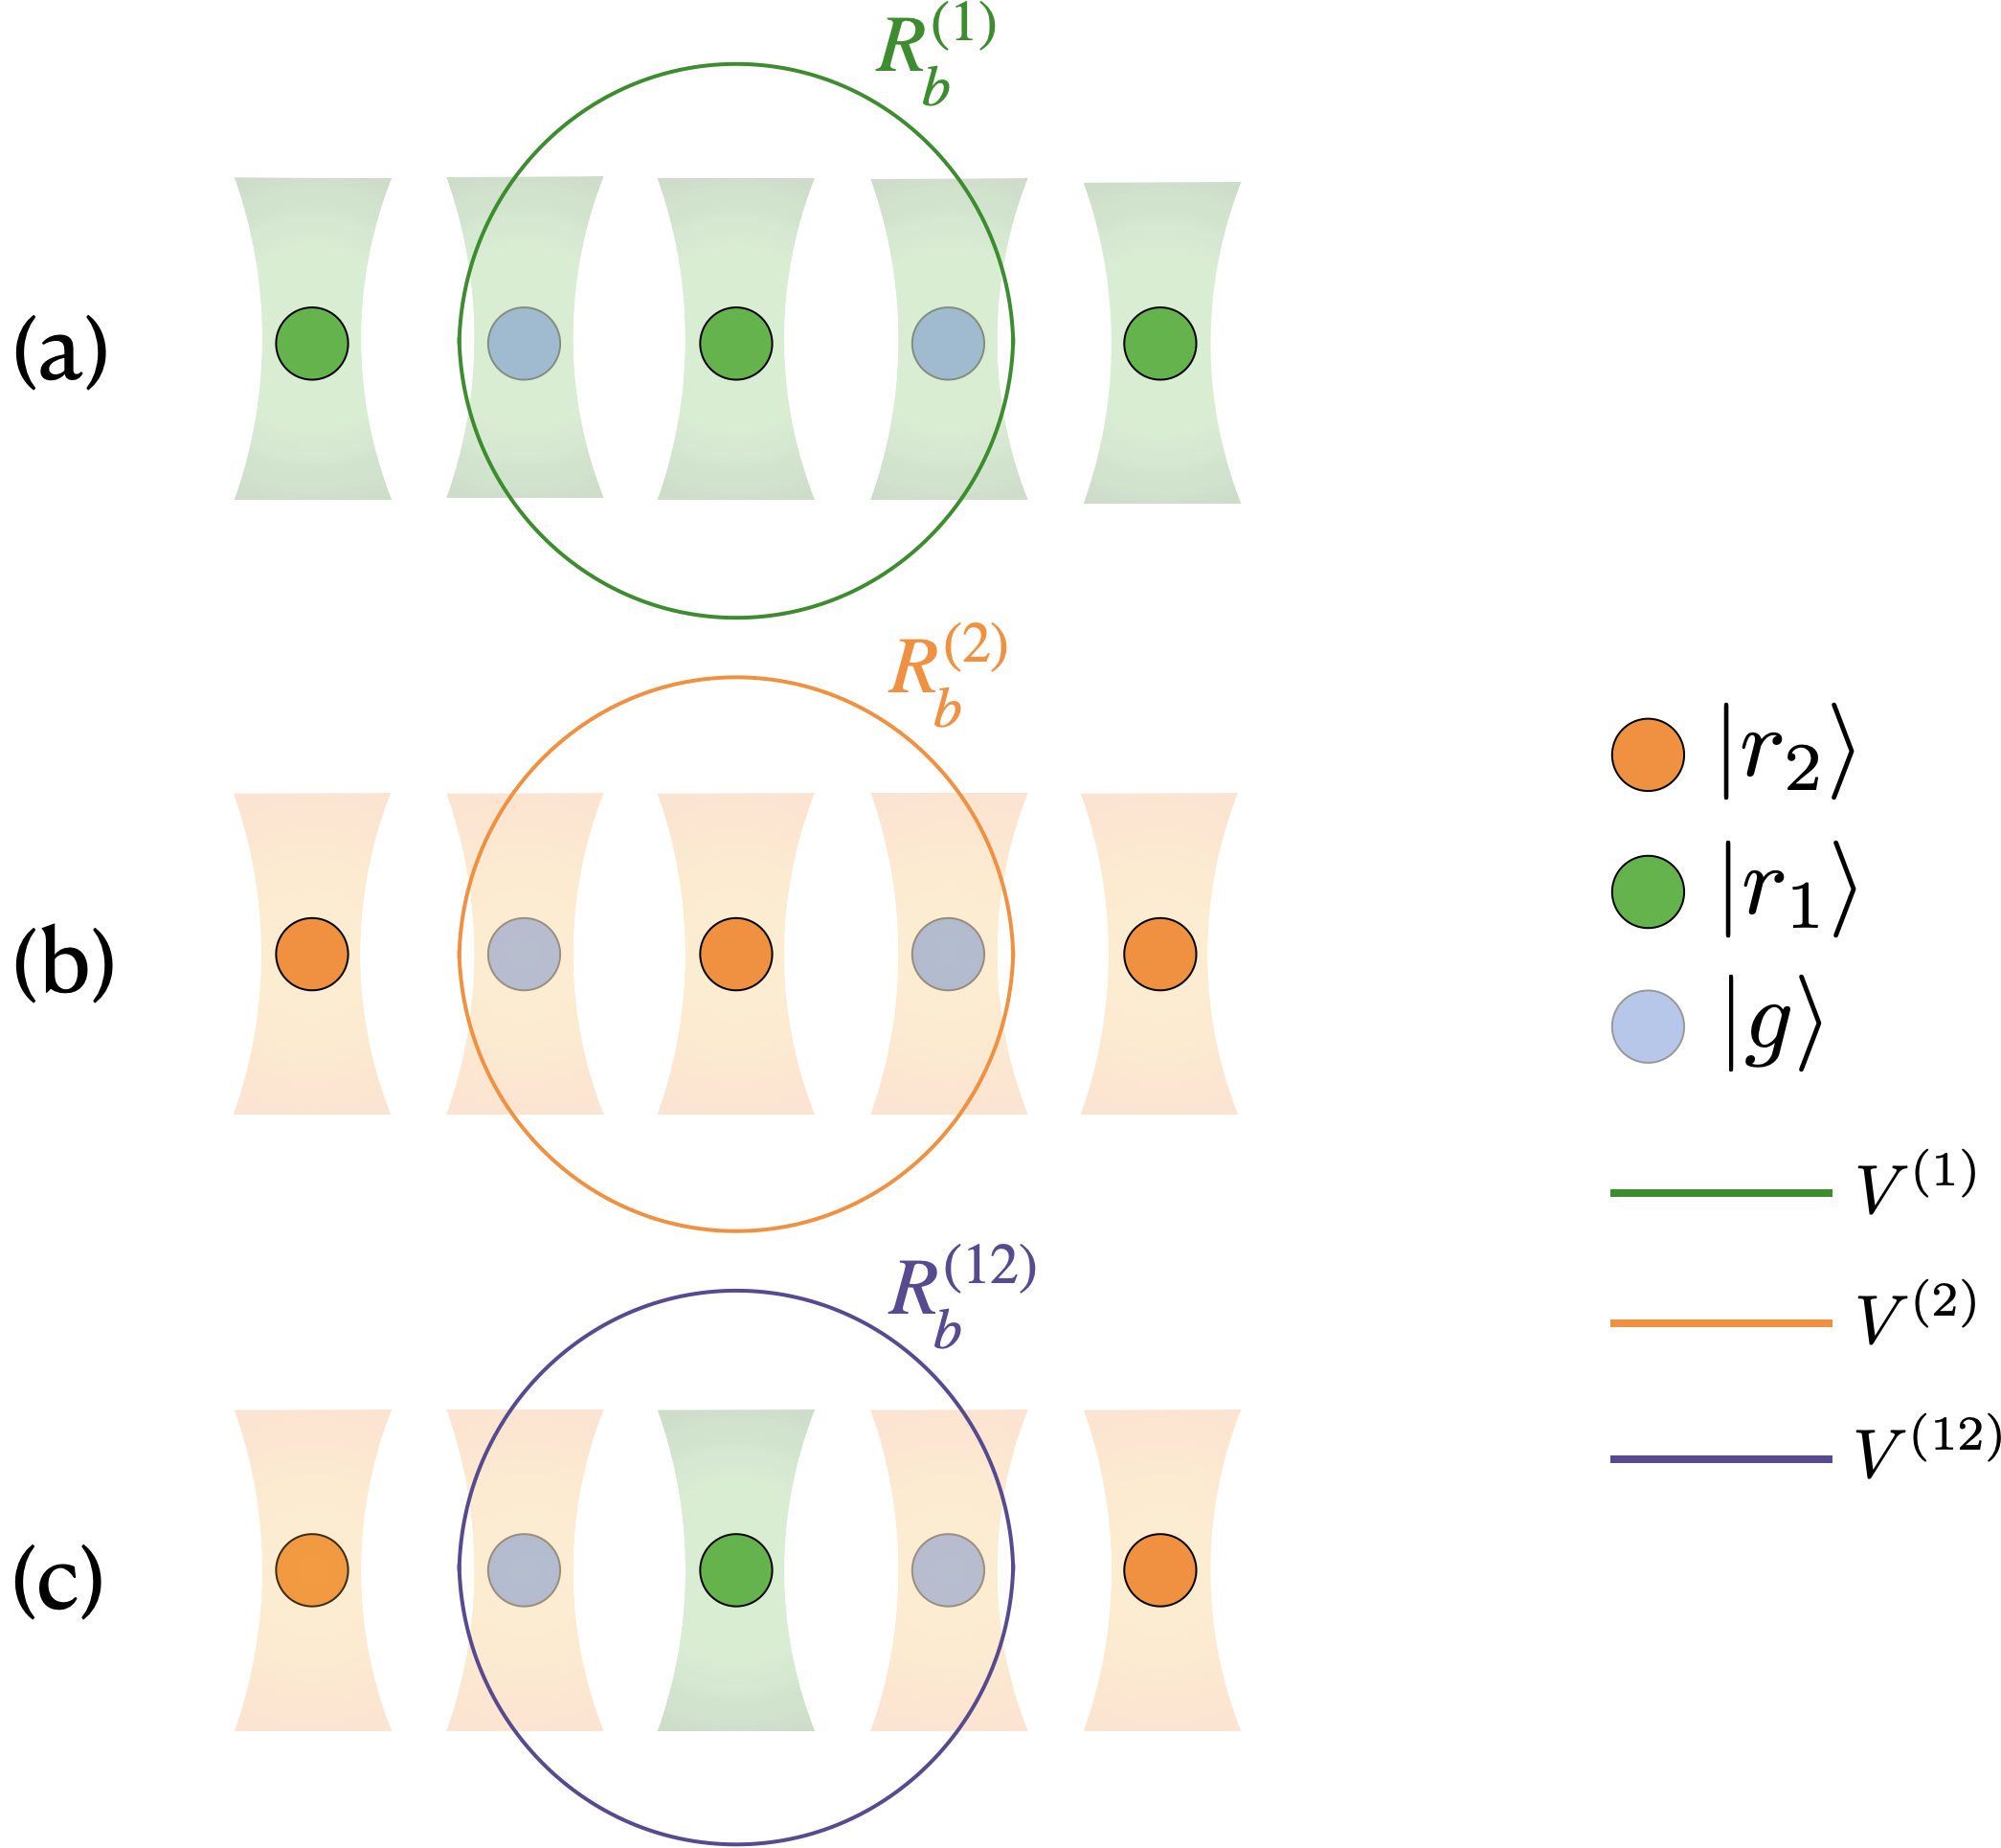
\includegraphics[width=8.5cm]{picture/Blockade_Mech.png}
    \caption{\textbf{The blockade mechanism between same Rydberg states.} (a) The $C^{(1)}_6$ interaction prevents neighbouring atoms within (green) radius $R^{(1)}_b = \sqrt[6]{|C^{(1)}_6|/\Omega}$ from being excited to same Rydberg state $\ket{r_1}$. (b) The $C^{(2)}_6$ interaction prevents neighbouring atoms within (orange) radius $R^{(2)}_b = \sqrt[6]{|C^{(2)}_6|/\Omega}$ from being excited to same Rydberg state $\ket{r_2}$. (c) The $C^{(12)}_6$ interaction prevents neighbouring atoms within (purple) radius $R^{(12)}_b = \sqrt[6]{|C^{(12)}_6|/\Omega}$ from being excited to different Rydberg state. In other words, the two green circles can never be seen together within green radius, similarly for two orange circles within orange radius. In contrast, two circles with different color can never be seen together within purple radius.}
    \label{fig:blockade}
\end{figure}\\

\emph{Rydberg crystals.}--- As in the previous work in \cite{Bernien2017ProbingSimulator} by Harvard group, the ground states of systems of Rydberg arrays, where each atom is coherently coupled to one Rydberg state (qubit), exhibit various many-body phases that break continuous translational symmetry. In these phases, the Rydberg atoms are arranged themselves to be in \emph{Rydberg crystals} which possess only discrete spatial symmetries with different orders, e.g., $\mathbb{Z}_2$-, $\mathbb{Z}_3$-ordered phases, corresponding to different Rydberg interaction strengths. The $\mathbb{Z}_2$ Rydberg crystal happens when $V_{i,i+1} \gg \Delta \gg \Omega \gg V_{i,i+2}$, indicating that the Rydberg blockade is effective for neighboring atoms but negligible for next-nearest neighbors. The Rydberg crystal therefore exhibits 2-site discrete translational symmetry. Similarly, the $\mathbb{Z}_3$ Rydberg crystal happens when $V_{i,i+1} \gg V_{i,i+2} \gg \Delta \gg \Omega \gg V_{i,i+3}$, indicating that the Rydberg blockade become even more effective up to the next-nearest neighbouring atoms. The Rydberg crystal therefore exhibit 3-site discrete translational symmetry. Both $\mathbb{Z}_2$ and $\mathbb{Z}_3$ Rydberg crystals are numerically shown in Fig.(\ref{fig:Z2-Z3}(b)), where we numerically calculate the ground state of 1D Rydberg arrays with open boundary condition (OBC) for $N=7$ atoms and then calculate the Rydberg fidelity for each atom as a bar plot. However, the situation turns out to be completely different for the system with OBC for $N=6$ atoms shown in Fig.(\ref{fig:Z2-Z3}(a)). In this case, the discrete spatial symmetries are jeopardized by the finite size effect, as the system size is too small such that the atoms in the bulk can be highly affected by the atoms at the boundary. This always happens for the systems of finite size that satisfy open boundary condition (OBC). To suppress such an effect, one can either study the systems in thermodynamic limit where $N \to \infty$, which is unlikely due to the limitation of computational resources, or employ periodic boundary condition (PBC). Yet, sometimes the OBC is favored, for instance, for efficiency of numerical methods such as the density matrix renormalization group (DMRG), one can instead employ the so-called smooth boundary condition suggested in \cite{Hikihara2011ConnectingDeformation}.  In this work, we propose alternative way of experimental realization that can circumvent the finite size effect caused by the boundary constraint and small number of system size, which will be explained in next paragraph. 
\begin{figure}[ht!]
    \centering
    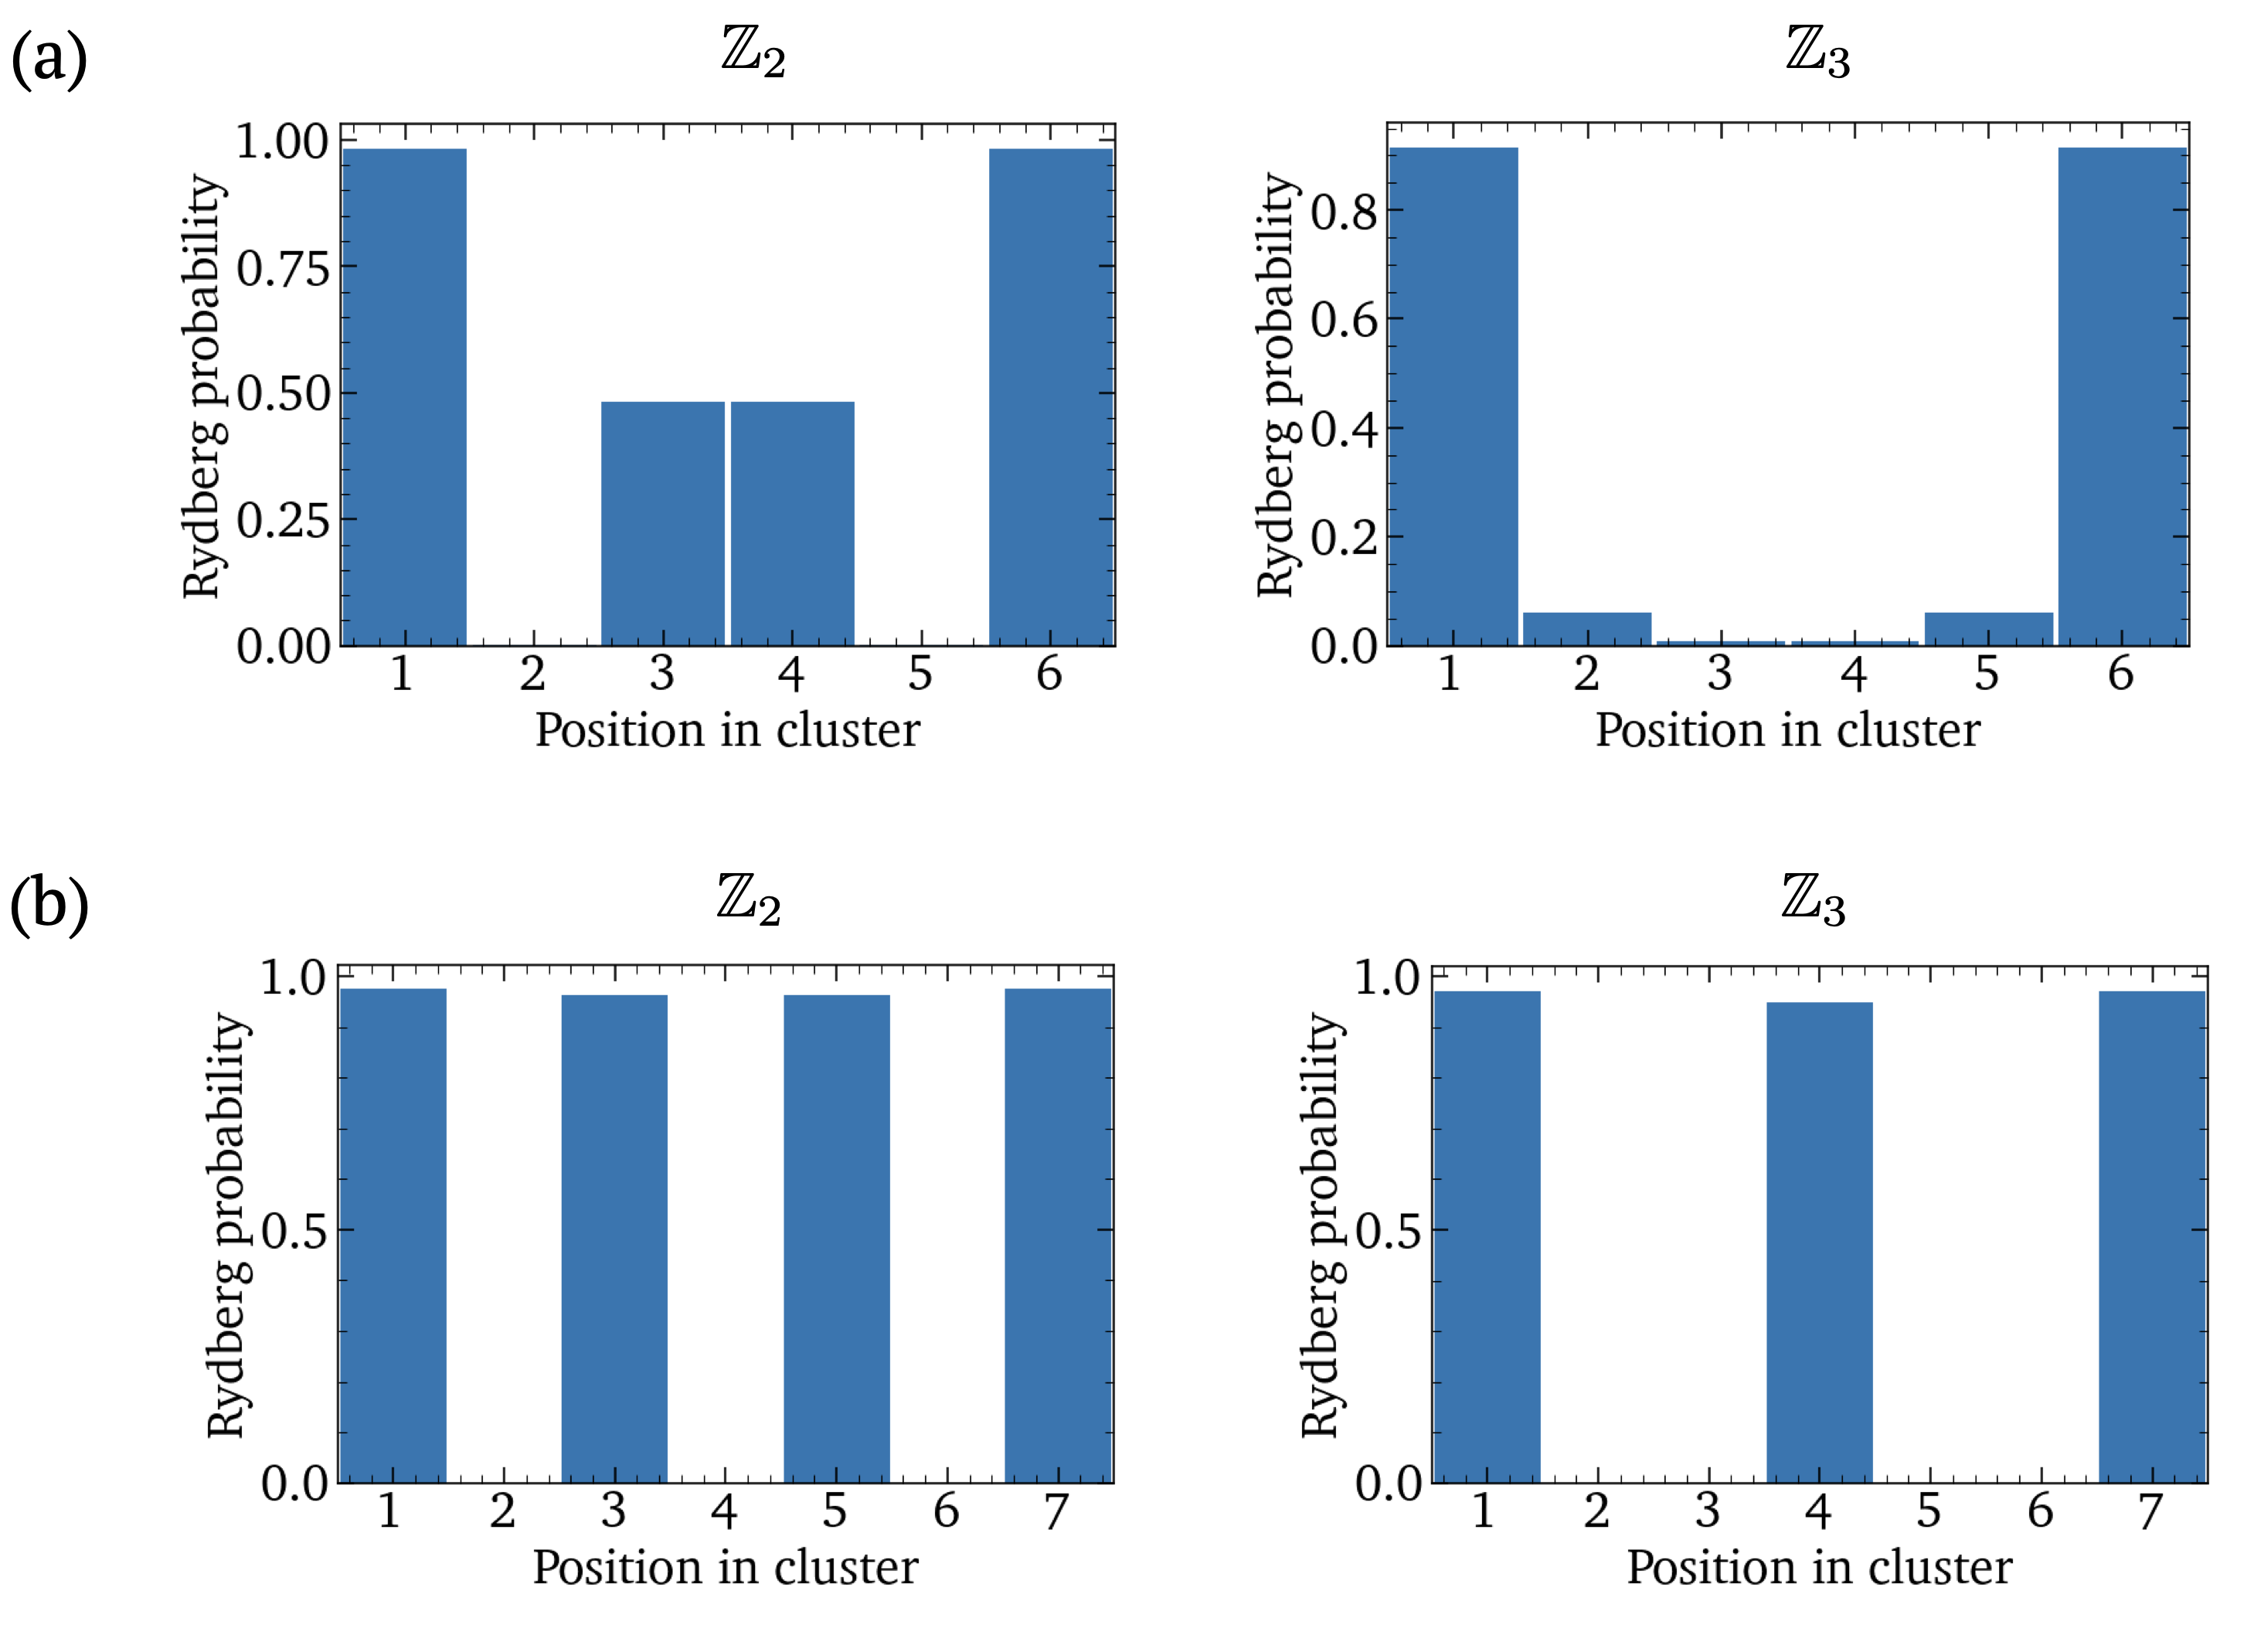
\includegraphics[width=8cm]{picture/Z2_Z3.png}
    \caption{\textbf{Rydberg crystals in system with OBC.} The ground state of system governed by Rydberg Hamiltonian in \cite{Bernien2017ProbingSimulator}, where $\mathbb{Z}_2$ and $\mathbb{Z}_3$ Rydberg crystals are formed when $a = 0.7R_b$ and $a = 0.4R_b$, respectively. (a) Both $\mathbb{Z}_2$ and $\mathbb{Z}_3$ Rydberg crystals are jeopardized in system with $N=6$, where the number of atoms is incommensurate with OBC. (b)  The formation of $\mathbb{Z}_2$ and $\mathbb{Z}_3$ Rydberg crystals are intact in system with $N=7$, where this number of atoms is commensurate with OBC. }
    \label{fig:Z2-Z3}
\end{figure}\\


\emph{Successive local driving technique.}--- 
\begin{figure*}[ht!]
    \centering
    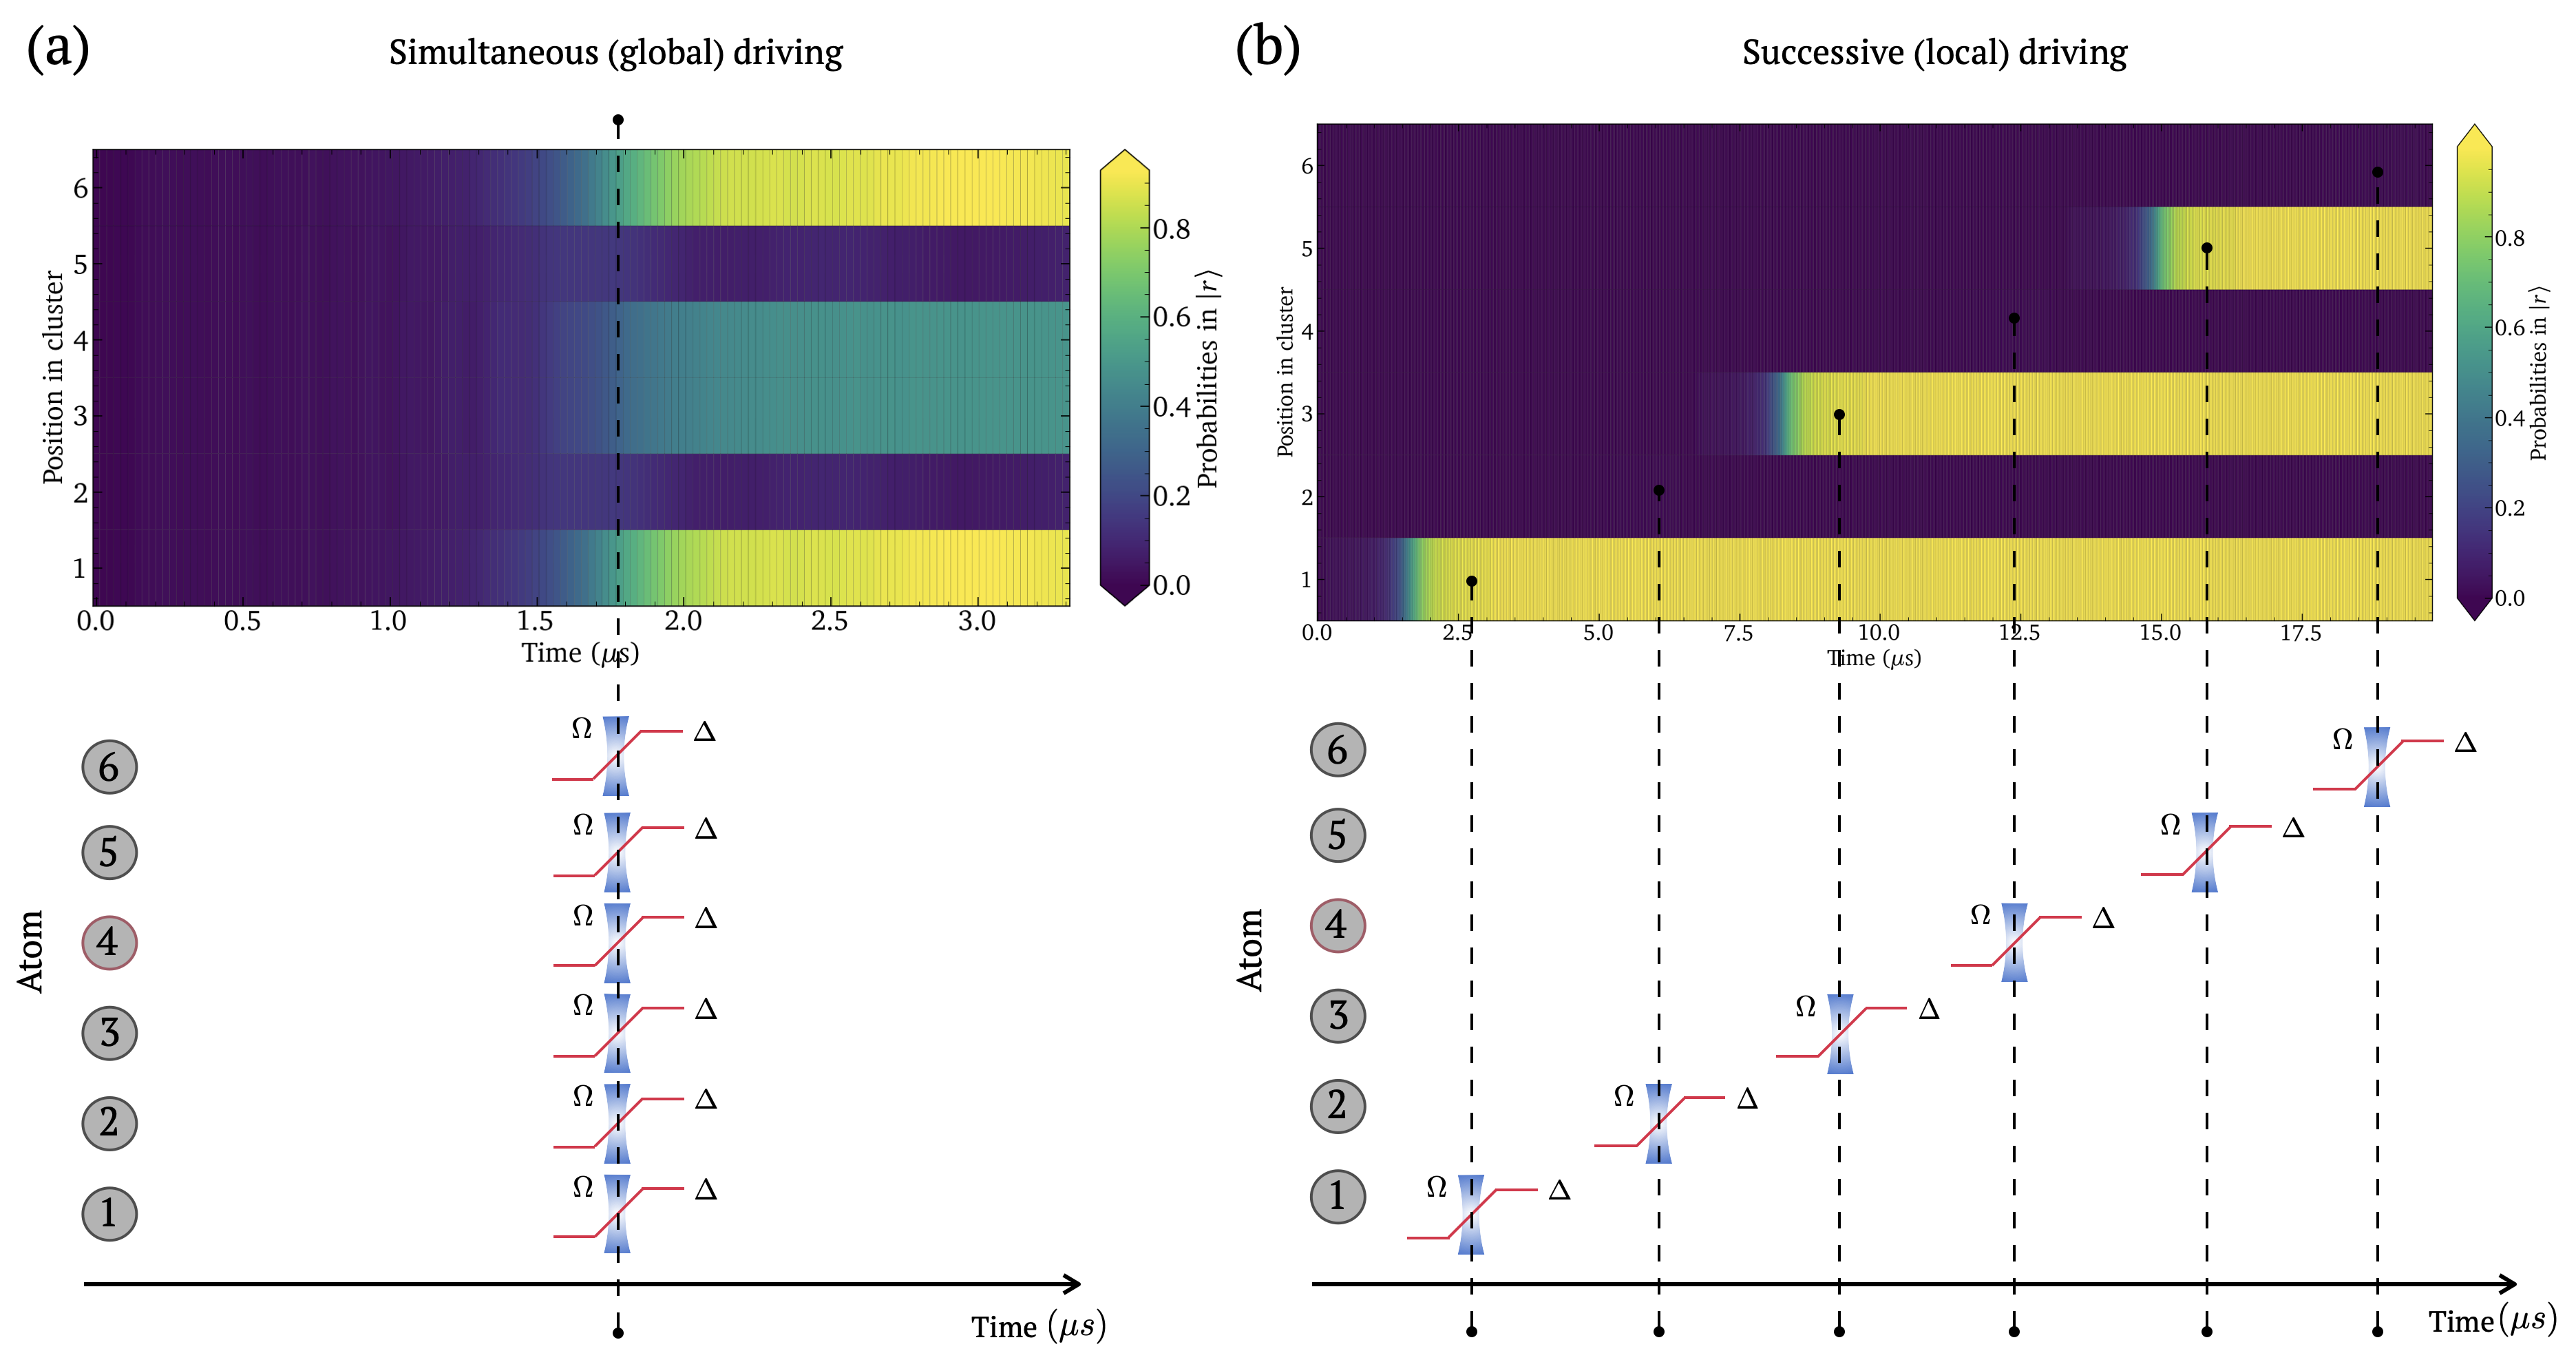
\includegraphics[width=14cm]{picture/successive_driving.png}
    \caption{\textbf{Successive local driving technique.} 1D Rydberg array with OBC for $N=6$ atoms are governed by the Rydberg Hamiltonian defined in \cite{Bernien2017ProbingSimulator}. To allow the $\mathbb{Z}_2$ crystal to form, we set lattice spacing $a = 0.7R_b$, where $R_b$ is blockade radius $R_b = (C_6/\Omega)^{1/6}$. Here, we choose the Rydberg state of Caesium (Cs) atom $80S1/2$ with $C_6 = 3199$ GHz $\mu m^6$, Rabi frequency $\Omega = 3 \times 2\pi \textit{\rm MHz}$, and detuning $\Delta = 10 \times 2\pi \textit{\rm MHz}$, which make $R_b=7.4 \hspace{1mm} \mu m$. We consider 2 cases when (a) Globally apply driving fields $\Omega(t)$ along with adiabatic sweepings of $\Delta(t)$ to all atoms at the same time, and (b) Locally applying driving fields $\Omega(t)$ along with adiabatic sweepings of $\Delta(t)$ in succession. The $\mathbb{Z}_2$ Rydberg crystal is jeopardized in (a) by the finite size effect with open boundary condition. However, to remedy this $\mathbb{Z}_2$ discrete spatial symmetry, one can perform successive local driving protocol as shown in (b) to ensure the formation of $\mathbb{Z}_2$ Rydberg crystal.}
    \label{fig:successinve_driving}
\end{figure*}
As mentioned above, in the system of finite size with OBC, the atoms in the bulk are highly sensitive to the atoms at the edges. Unfortunately, the traditional protocols of Rydberg quantum annealing are implemented via quantum adiabatic evolution where all driving parameters, i.e., detuning $\Delta$ and Rabi frequency $\Omega$ are slowly changed in time and simultaneously applied for a global. Owing to weak interaction of atoms at the chain's end, leading to greater suppression of an energy shift compared to the others in the bulk, causing them to be definitely excited to the Rydberg state regardless of other excitations. As numerically demonstrated in Fig.(\ref{fig:successinve_driving}(a)), we consider the system with OBC for $N=6$ atoms with the lattice spacing being tuned by $a = 0.7R_b$. In PBC consideration, the system normally manifest $\mathbb{Z}_2$ crystal structure. However, such a structure is destroyed in the system with OBC. This happens due to global simultaneous driving guarantees the Rydberg excitation for the atoms at the chain's end, which energetically prohibit the Rydberg excitations of the atoms in the bulk. Therefore, in order to allow the $\mathbb{Z}_n$ Rydberg crystals to form, one need to be aware of the number of system size being commensurate with corresponding $\mathbb{Z}_n$ structure in OBC. For instance, the $\mathbb{Z}_2$-ordered phase is commensurate with the system sizes of $N=3,5,7,9,...$, etc., and the $\mathbb{Z}_3$-ordered phase is commensurate with the system sizes of $N=4,7,10,13,...$,  etc. Owing to this, both $\mathbb{Z}_2$ and $\mathbb{Z}_3$ crystals are jeopardized in the Rydberg array with $N=6$ atoms in OBC. On the other hand, the Rydberg array with $N=5$ atoms is only allow for $\mathbb{Z}_2$ crystals to form. To circumvent this effect, we propose an alternative experimental protocol called \emph{successive local driving} which is explicitly shown as in Fig.(\ref{fig:successinve_driving}(b)). In this protocols, we take turns on performing local driving of Rabi frequency $\Omega(t)$ along with adiabatic sweeping of detuning $\Delta(t)$ for one atom after another starting from the first atom. This prevents another atoms at the chain's end from being excited to Rydberg states, allowing Rydberg excitation to occur in the right places for corresponding $\mathbb{Z}_n$ structure ($\mathbb{Z}_2$ in this case). In Fig.(\ref{fig:successinve_driving}(b)), we found that at the end of the protocol, the $\mathbb{Z}_2$ Rydberg crystal is recovered in spite of the fact that the system is small size and satisfies OBC. However, this protocol also has a fundamental disadvantage, which is to take much longer time for one cycle of the protocol. Fortunately, this experimental realization is still rational due to long Rydberg life time up to 200 $\mu s$, which is much longer than time duration used in one complete loop of the protocols, however, depending on the number of atoms and chosen Rydberg states.  

 
\subsection{Graph coloring problem on unit disk graph (GCP-UD)}

Using quantum simulator with Rydberg atoms to solve combinatorial optimization problems is one of the most prominent applications in the field of quantum optimization. One of the very famous problems is maximum independent set (MIS) on unit disk graph (UDG). The so-called unit disk graph is defined as a graph $G=(V,E)$ with sets of vertices $V$ and edges $E$ such that any two vertices can only be connected by an edge if and only if they are separated by a distance smaller than a unit radius. The MIS problem on this graph is then defined as a largest subset of vertices in which no pair is connected. The Rydberg-atom quantum simulator benefits from Rydberg blockade mechanisms, which provide natural connection with unit disk graph where the unit radius is identified with Rydberg blockade radius. In this work, we introduce another class of optimization problems that can be solved by Rydberg-atom quantum simulators, which is called \emph{graph coloring problem} (GCP) \\

\emph{Graph coloring problem (GCP).}--- Given an undirected graph $G=(V,E)$, where $V$ is a set of vertices and $E$ is a set of edges, graph coloring is a way of labelling all vertices such that no pair of adjacent vertices are assigned the same color. A graph coloring that use at most $k$ different colors is called k-coloring, and the minimum number of colors required to color the graph is called its \emph{chromatic number} $\chi(G)$. The mathematical definition of k-coloring is then followed by
\begin{definition}
\label{def:k-coloring}
{\rm (k-coloring)} For an undirected graph $G = (V,E)$, the k-coloring is a mapping $f_k: V(G) \to \mathbb{C}_k$ with $f(v)\neq f(w)$ for all $(v,w) \in E(G)$. Here, $\mathbb{C}_k = \{1,2,...,k\}$ is a set of k colors.
\end{definition}
The number $f(v)$ is called the color of a vertex $v$. The graph coloring is then to partition all the vertices into different $k$ \emph{stable set} corresponding $k$ different colors. The graph coloring problem is defined as 
\begin{definition}
\label{def:k-color}
{\rm (graph coloring problem)} For an undirected graph $G = (V,E)$, the task is to find a k-coloring  $f_k: V(G) \to \mathbb{C}_k = \{1,2,..,k \}$ of $G$ with minimum $k$
\end{definition}
In other words, the problems aim to find the smallest number of color (chromatic number $\chi(G)$) of a graph). This problem is known to be NP-hard \cite{Garey1976TheColoring}. The solution is sometimes called optimal graph coloring in which there exists k-coloring where $k=\chi(G)$. However, this problems are in general very difficult to solve, the problems are then relaxed to finding the k-coloring where $\chi(G)\leq k \leq |V|$, which is known to be NP-complete \cite{Karp1972ReducibilityProblems}. In this case, the graph coloring is called non-optimal. The examples of graph coloring is explicitly demonstrated as in Fig.(\ref{fig:graph_coloring})
\begin{figure}[ht!]
    \centering
    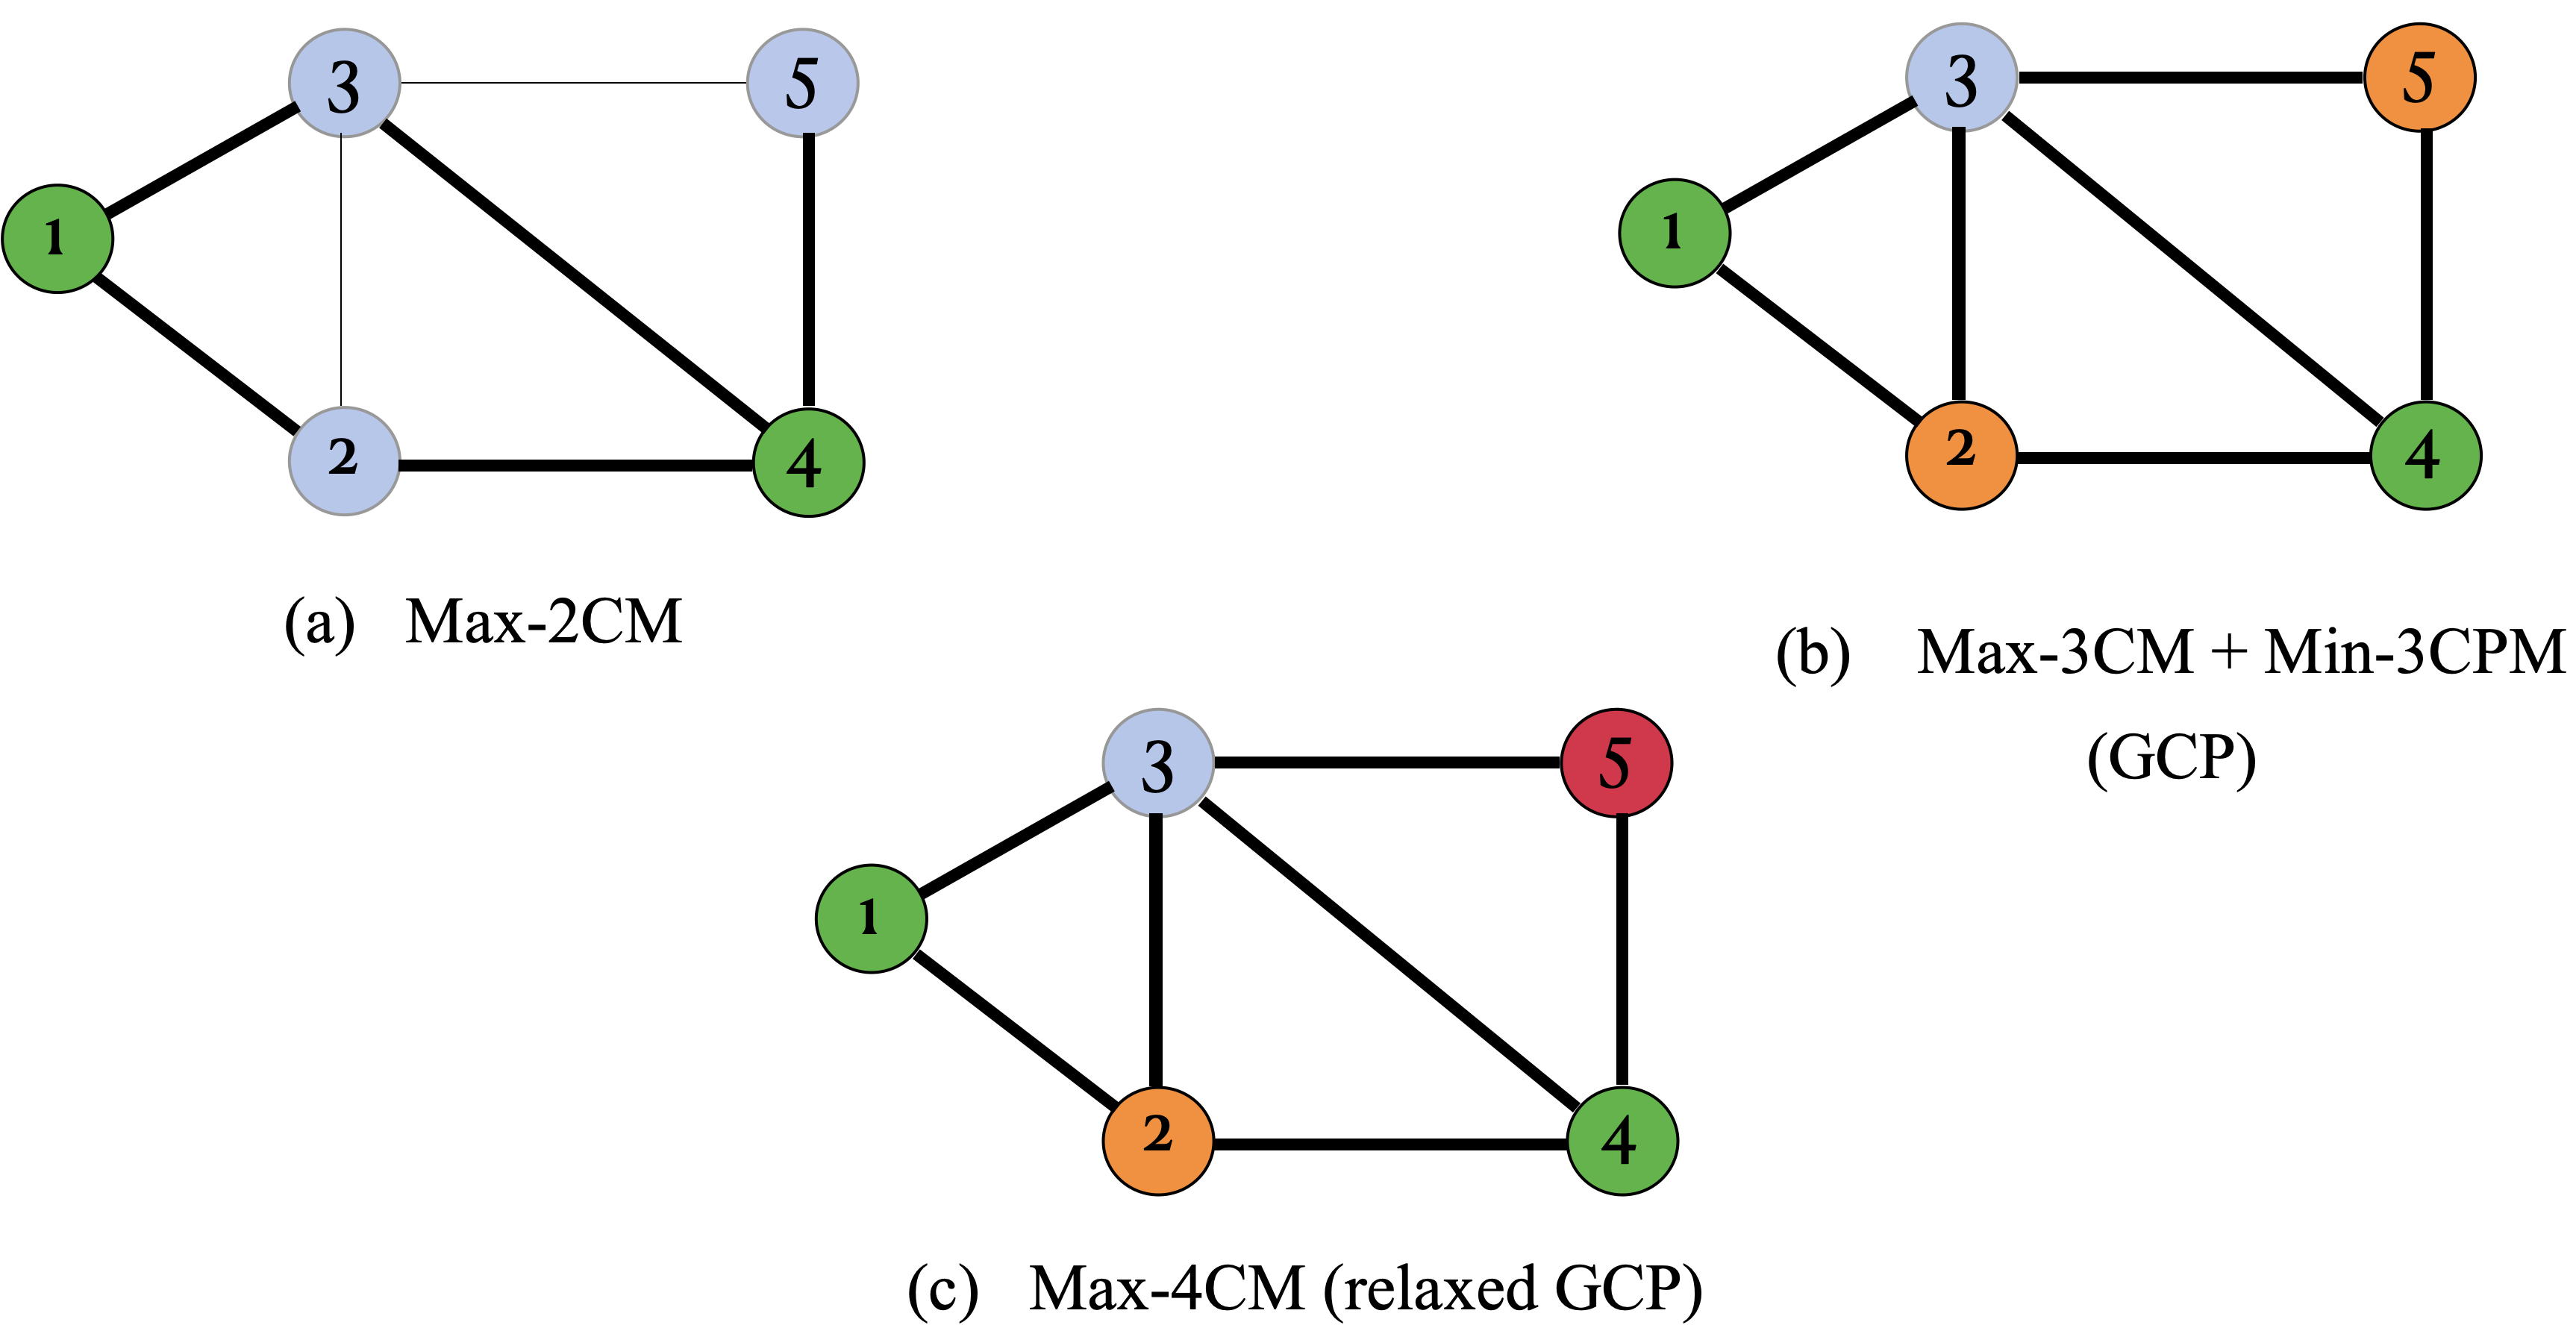
\includegraphics[width=8.5cm]{picture/color_matching.png}
    \caption{\textbf{The examples of graph coloring.} (a) Invalid graph coloring as there are adjacent vertices , i.e., \{(2,3),(3,5)\}, that share the same color. (b) The graph coloring is valid in the sense that all adjacent vertices are assigned with different colors. Besides, it is an optimal as one can never found the coloring of this graph with the number of colors less than 3. The \emph{chromatic number} of this graph is therefore equal to 3. i.e., $\chi(G)=3$. (c) The graph coloring is valid but not optimal as the number of colors used is 4, which is greater than the chromatic number. Sometimes is said to be relaxed graph coloring.} 
    \label{fig:graph_coloring}
\end{figure}\\


\emph{Mapping problem graph onto Rydberg-qutrit interaction graph.}--- Given the advantages of optical tweezers, one can move atoms adiabatically such that the graph structure is changed. The example is demonstrated in Fig.\ref{fig:graph_mapping}, where we consider the interaction regime of $R^{(1)}_b:R^{(2)}_b:R^{(12)}_b=1:1:0.5$. With mobile lattice spacing $a$ featured by the use of optical tweezers, one can define the structure of unit disk graphs on which optimization problems depend. Since we identify the unit radius of such a unit disk graph with the largest blockade radius, which in this case is $R^{(1)}_b$, meaning that any atoms within this range of radius are connected by interaction. For $a = 0.8R^{(1)}_b$, each atom can only connect to a nearest atom as the blockade only cover the nearest atom (Fig.\ref{fig:graph_mapping}(a)). However, bringing each atom closer to each other, saying $a = 0.4R^{(1)}_b$, make the blockade range reaches the next nearest atom, connecting atom $i$ to atom $i+2$ as well (Fig.\ref{fig:graph_mapping}(b)). In the terminology of graph, we say that the vertices (atom) in Fig.\ref{fig:graph_mapping}(a) have at most 2 degrees of freedom, i.e., the maximum number of edges incident to the vertex is 2, whilst the vertices in Fig.\ref{fig:graph_mapping}(b) have at most 4 degrees of freedom. In this graph mapping paradigm, arbitrary 2D unit disk graphs can be mapped onto 1D Rydberg-qutrit arrays. 
\begin{figure}[ht!]
    \centering
    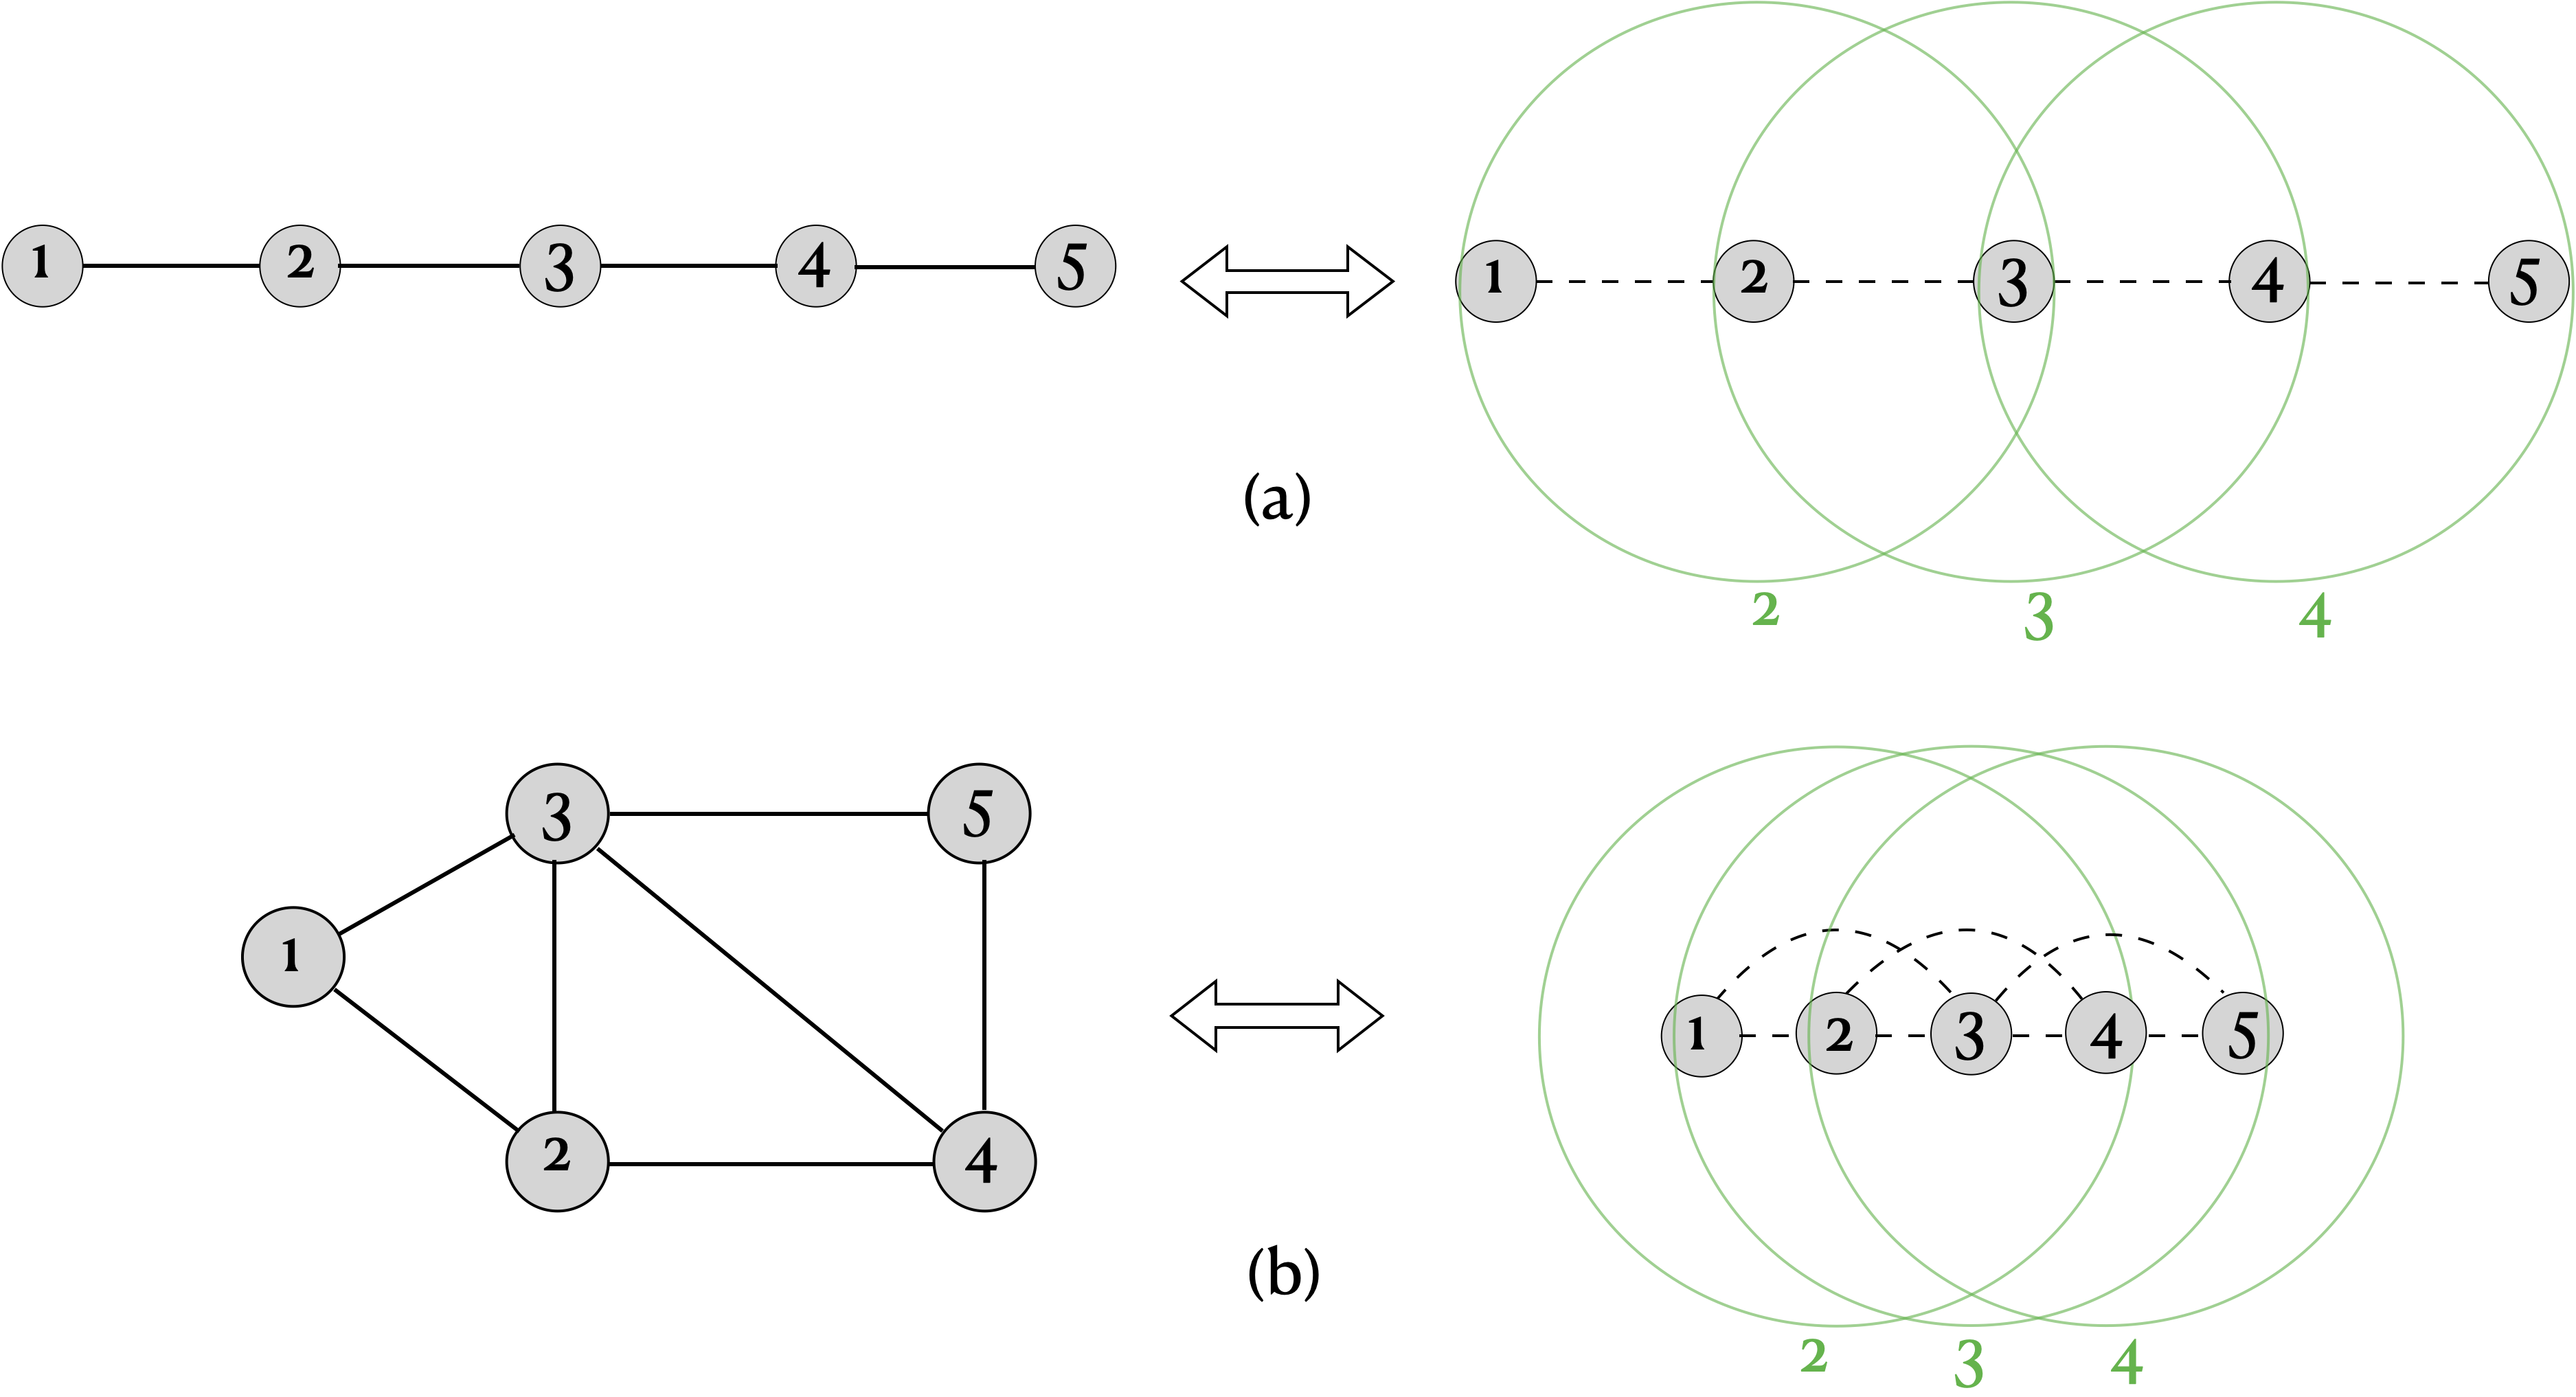
\includegraphics[width=8cm]{picture/graph_mapping.png}
    \caption{\textbf{Mapping problem graph to Rydberg-qutrit interaction graph.} The left panel shows random UDGs from problem graphs, consisting of vertices connected by edge (solid line). The right panel show the Rydberg-qutrit array with all interactions between atoms (dash line). (a) $a = 0.8R^{(1)}_b$,  (b) $a=0.4R^{(1)}_b$. When each atom come closer to each other as in (b) the blockade range is extended beyond the nearest atom and reach the next nearest atom. which make atom $i$ also connect to atom $i+2$ not just only atom $i+1$ as shown in (a). The green circles represent the blockade radius generating from atom 2, 3, and 4, respectively.}
    \label{fig:graph_mapping}
\end{figure}

\subsection{Two detuning sweeping in time order}

\begin{figure*}[b!]
    \centering
    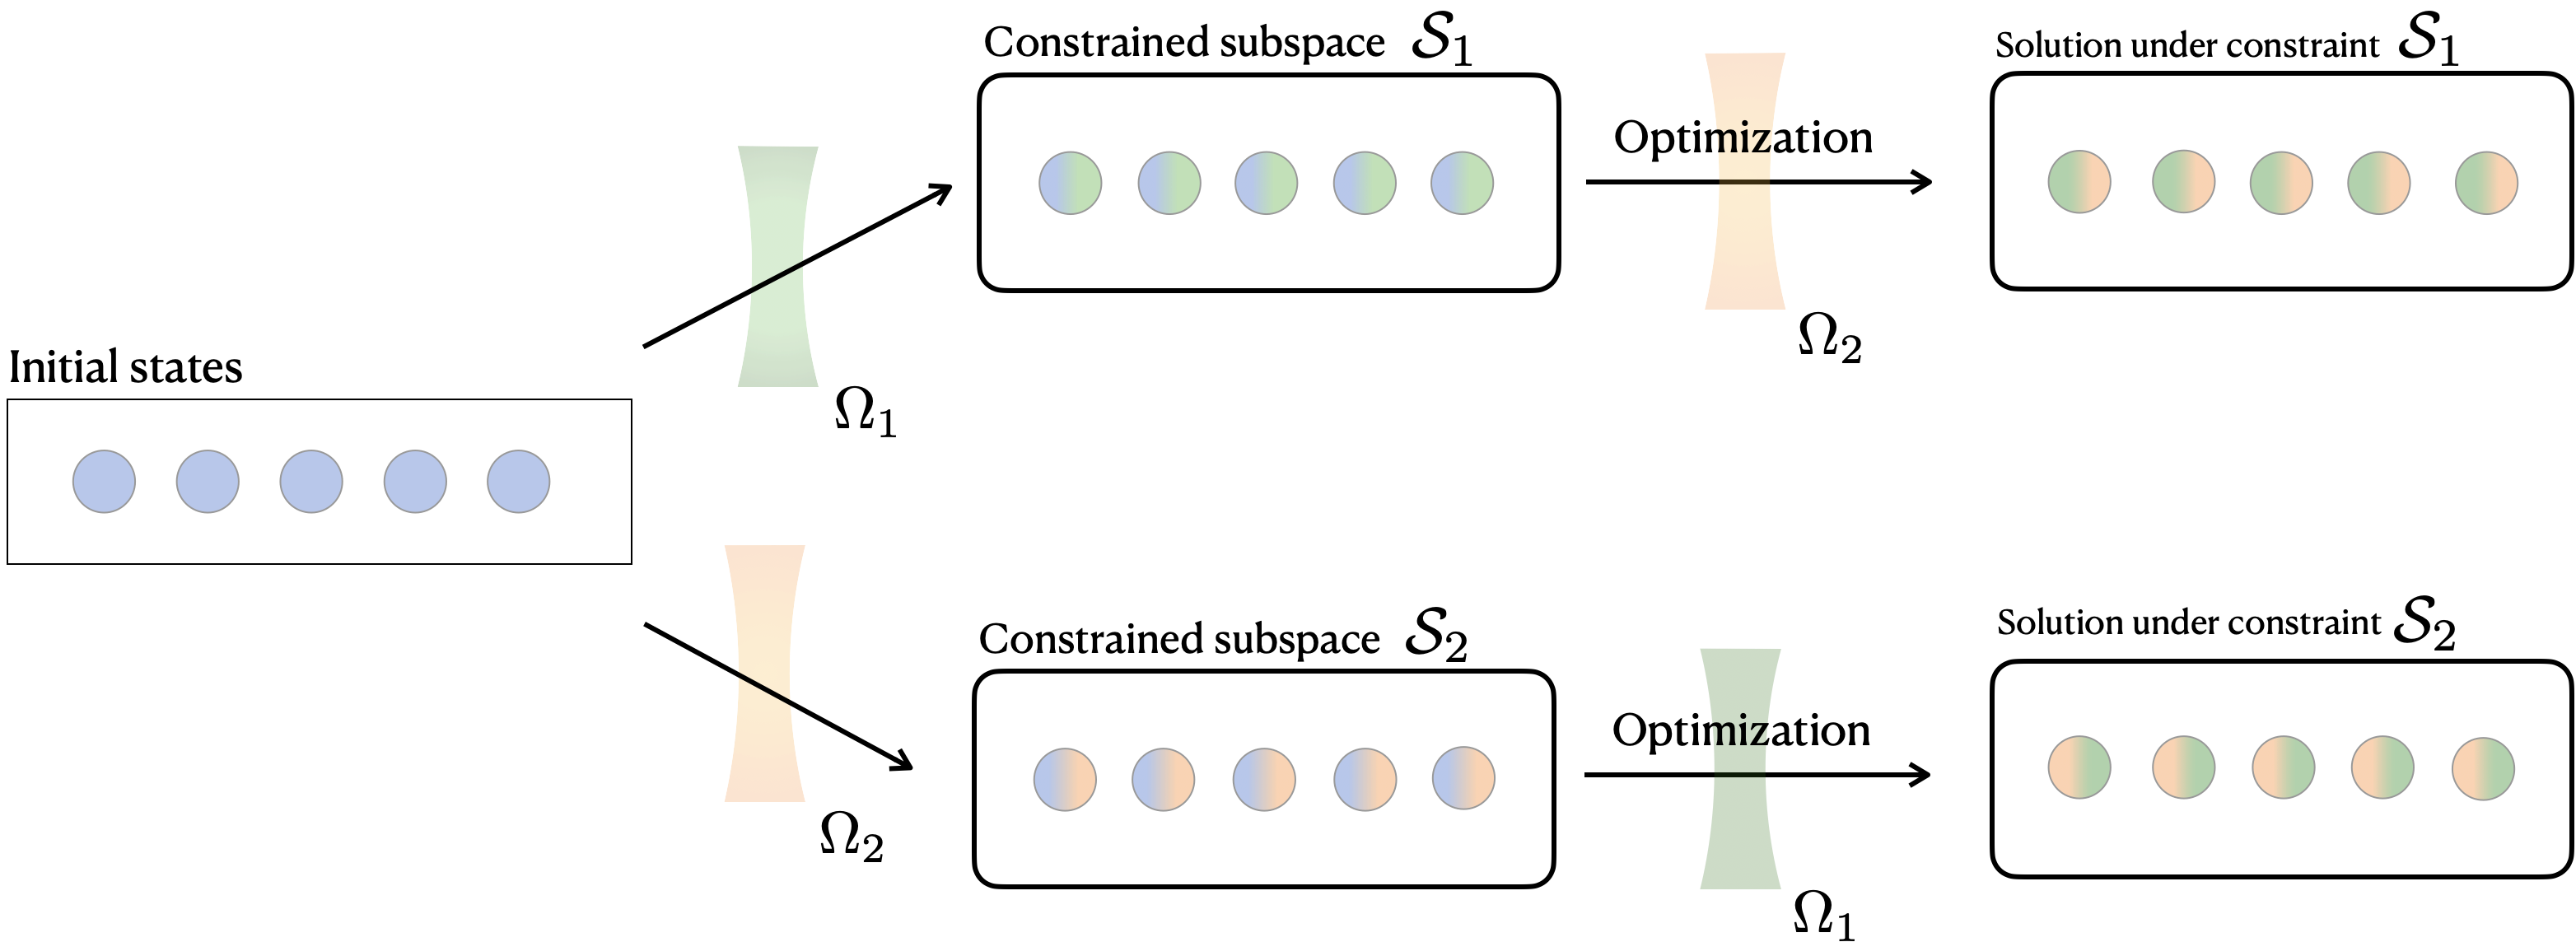
\includegraphics[width=12cm]{picture/opti_procedure.png}
    \caption{\textbf{Detuning sweeping in order}.  The diagram shows the procedures along each sequential detuning sweeping. The first sequential sweeping (above procedure) is to encode the associated constraint of the annealing state being in $\mathcal{S}_1$ by first sweeping $\Delta_1(t)$ to drive the annealing state into subspace $\mathcal{S}_1$, and then carry on the optimization by sweeping $\Delta_2(t)$ to drive the final state to be the solution to the optimization under constraint $\mathcal{S}_1$. Vice versa for the second sequential sweeping (below procedure).}
    \label{fig:opt_procedure}
\end{figure*}
In general, the real-world optimization problems are always attached by certain constraints, the problems can traditionally be solved by relaxing hard constraints by putting them into cost functions and only easy constraints are left, e.g., method of Lagrange multiplier, Lagrangian relaxation, etc., making the problems much easier to be solved in spite of the fact that it will lead to the greater number of decision variables in cost functions. In the regime of quantum optimization using QAA with Rydberg-atom qutrit quantum optimizer, we offer a new optimization protocol which allows associated constraints to be encoded along the process of QAA. Such a protocol utilize the fact that there are multiple coherent drivings to multiple Rydberg states inside each individual atoms such that the atom array can be driven into various low energy subspaces, and desired optimization constraints can be characterized by such subspaces. In this section, we consider 2 cases of $C_6$ interaction regimes as the following:



\section{Results}

We consider the quantum optimizer with Rydberg-atom qutrits for $N = 5$ atoms. Here, we show how to use such an optimizer with QAA to solve various problems of Max-kCM and Min-kCPM. One of the main advantages of this optimizer lies in the variety of Rydberg states that can be chosen for various optimization tasks. However, it is necessary for one to choose proper Rydberg states $\ket{r_1}$ and $\ket{r_2}$ to solve a specific optimization. In this work, we show a few numerical showcases of optimization for Max-kCM and Min-kCPM with different scales of interaction strength between $R^{(1)}_b$, $R^{(2)}_b$, and $R^{(12)}_b$. It has been found that there are two key features of this quantum optimizer with Rydberg-atom qutrits from which the optimization can benefit.The first feature is that different orders of detuning sweeping for $\Delta_1$ and $\Delta_2$ can effectively yield solutions to optimization under different constraints, more specifically the first detuning sweeping imposes certain constraints on the annealing quantum state, and the second sweeping carries on the optimization under such constraints. The second feature is due to the coexistence of three species of Rydberg blockades, one can make use of optical tweezers to allocate each atom separated by different lattice spacings within these blockades, such that the interaction graph (still a UDG), i.e. the graph of the optimization problem, can be tuned into the way that suits the optimization. 


\subsection{1D-array}
\begin{figure*}[t!]
    \centering
    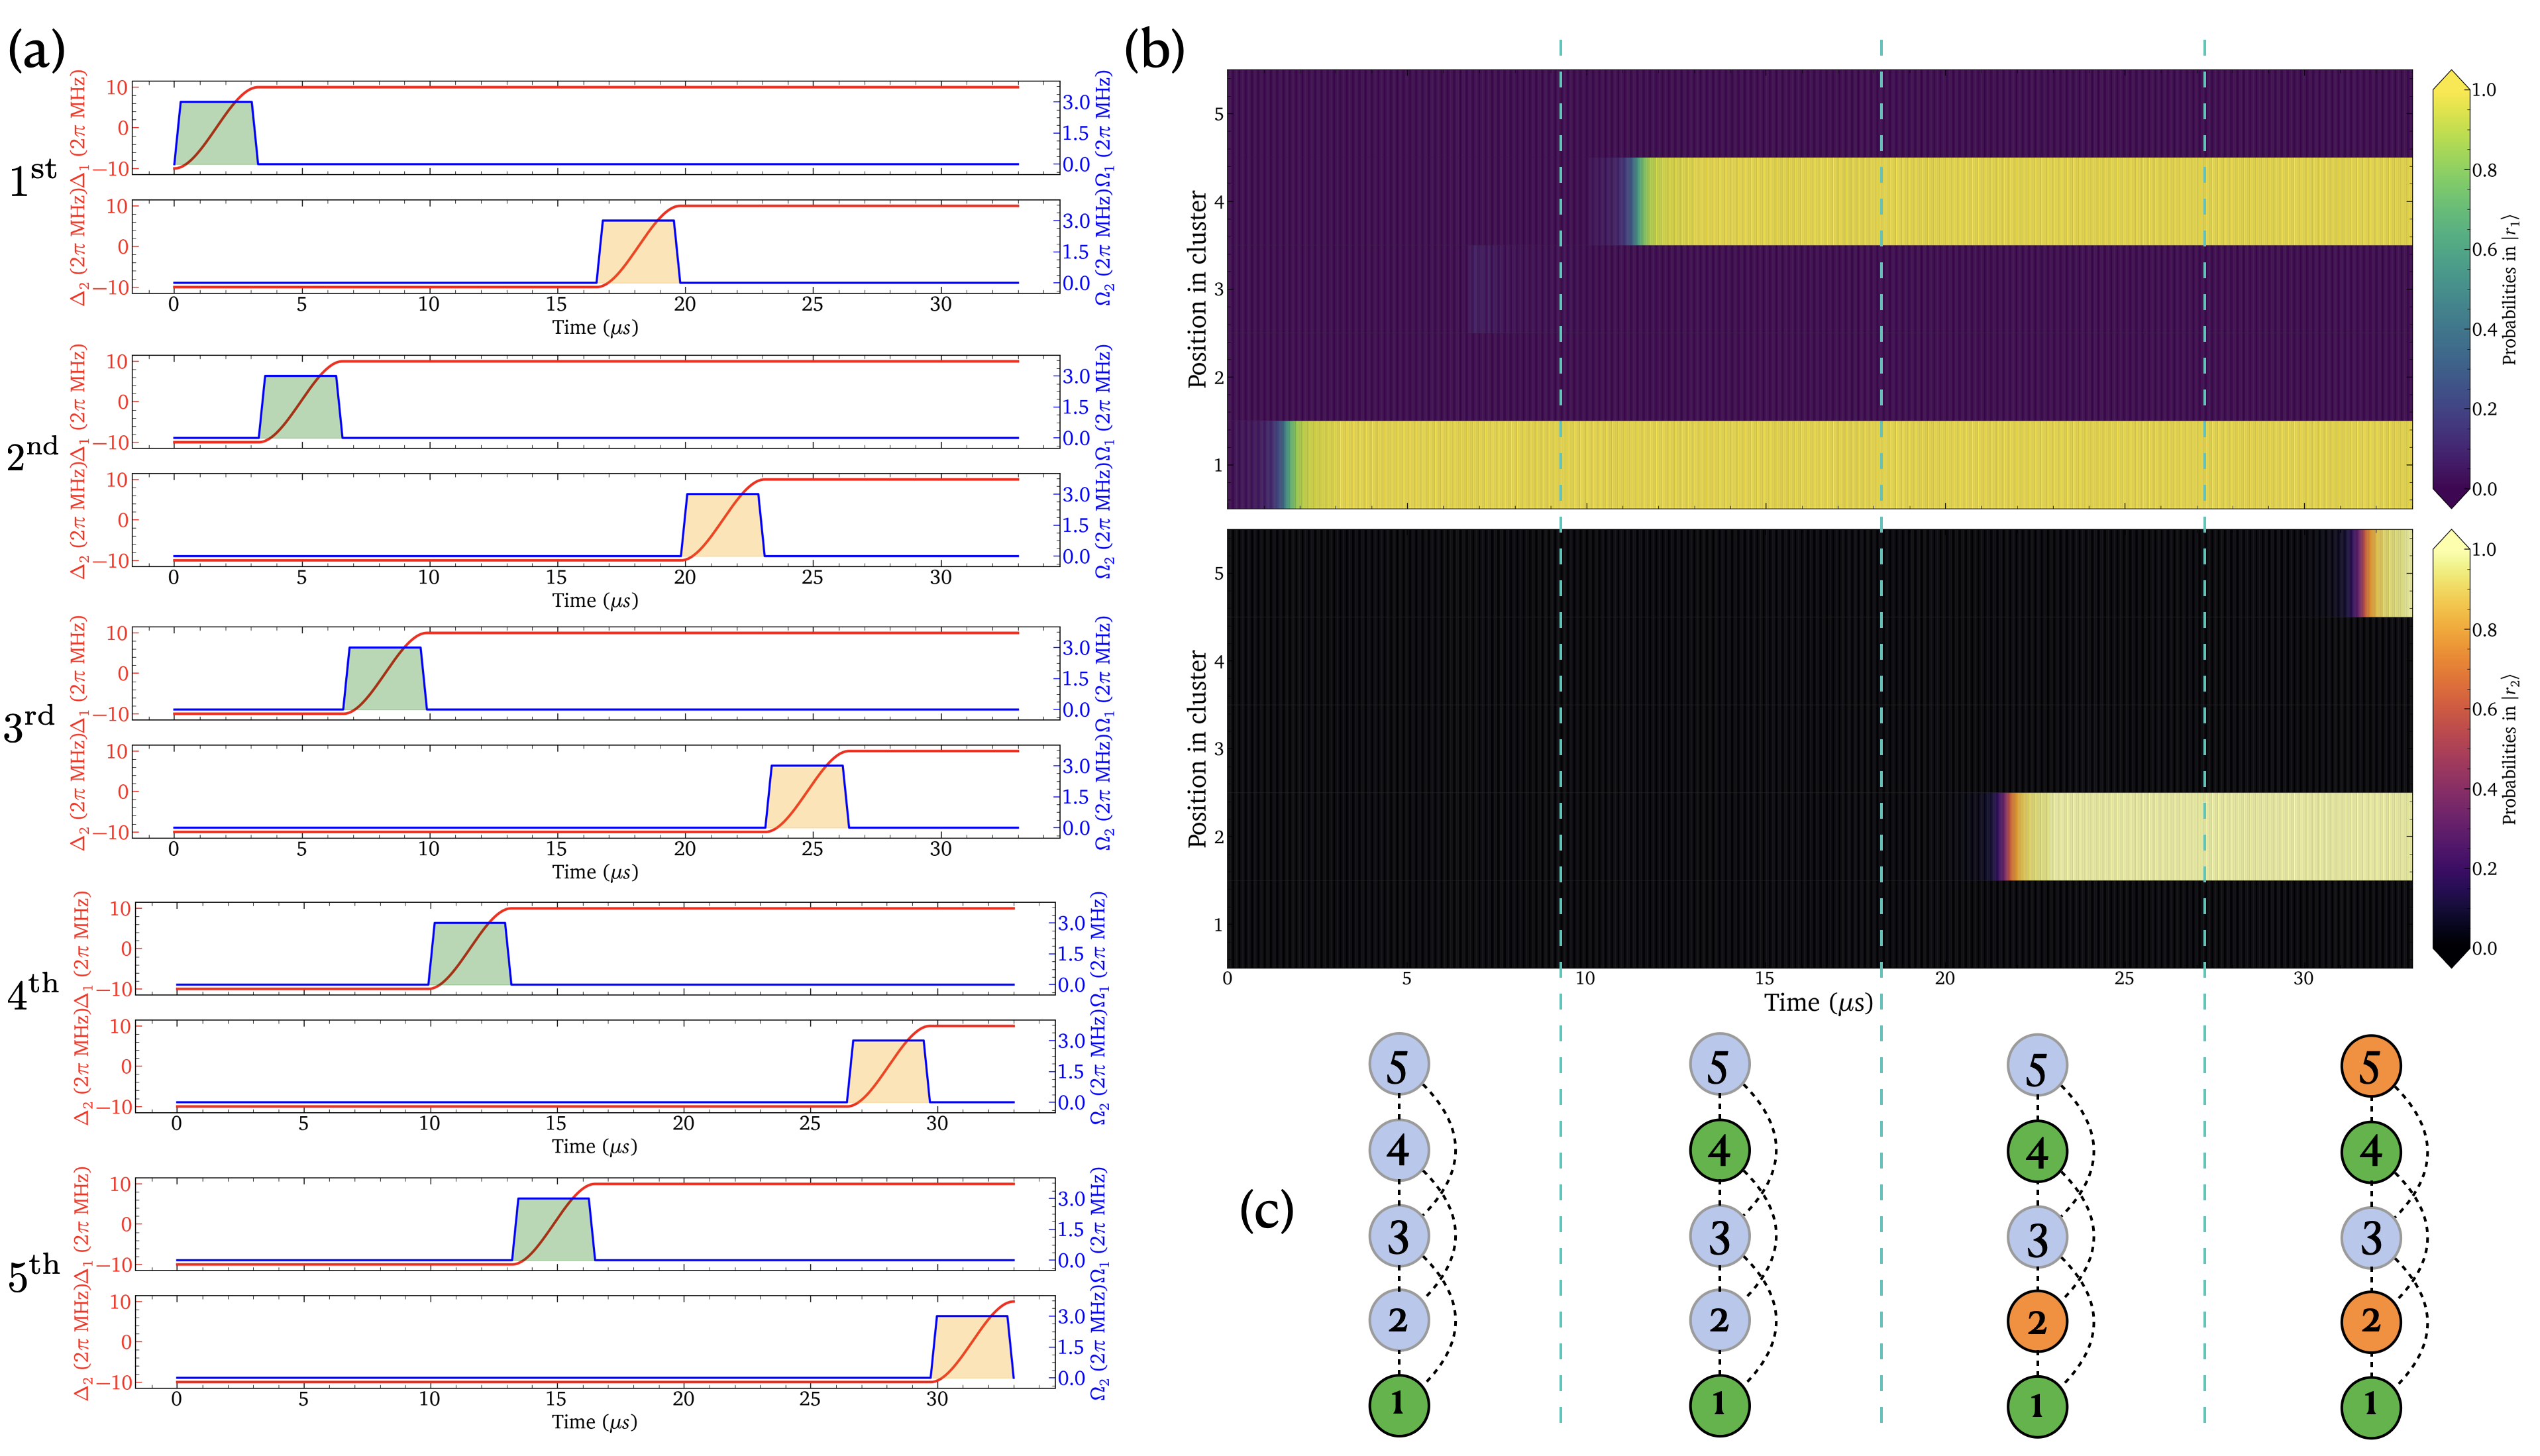
\includegraphics[width=13cm]{picture/GCP_5atom.png}
    \caption{\textbf{GCP 5 atoms} }
    \label{fig:case1_ultimate}
\end{figure*}

\subsection{2D-array}
\begin{figure*}[t!]
    \centering
    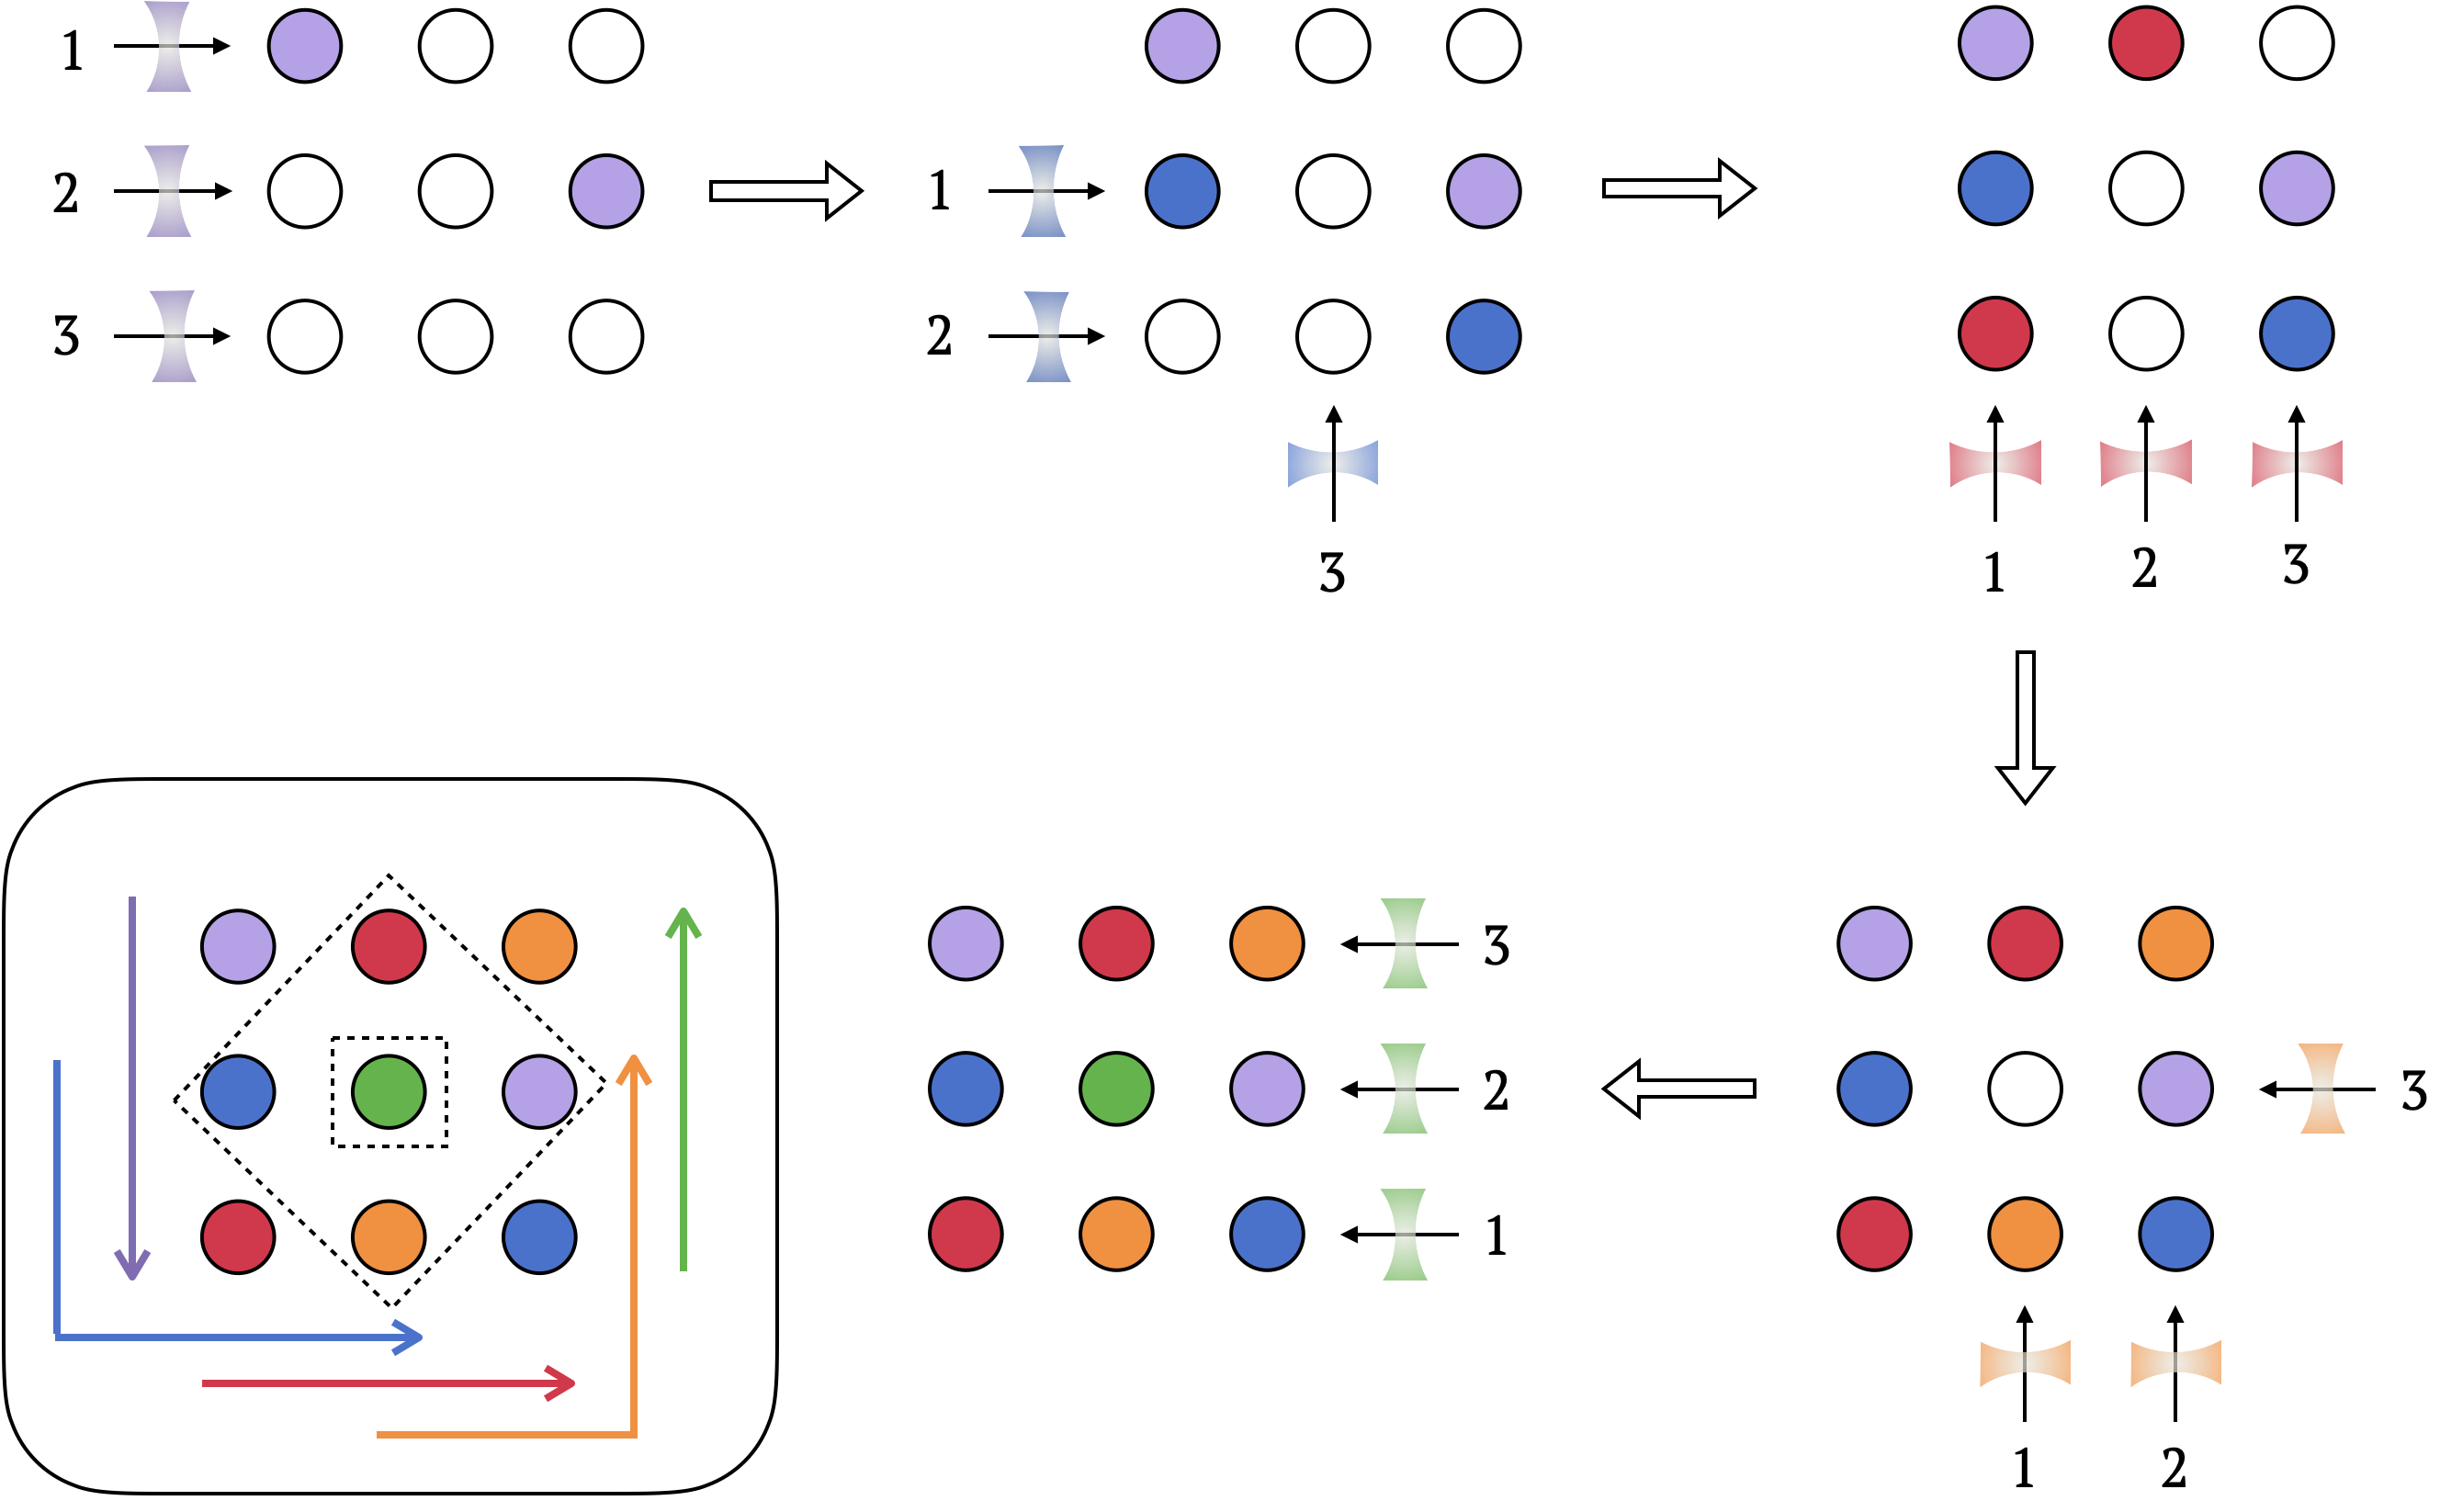
\includegraphics[width=13cm]{picture/GCP_2D.png}
    \caption{\textbf{GCP in 2D array} }
    \label{fig:case1_ultimate}
\end{figure*}


\section{Conclusion}
The optimization protocols developed in this work can be understood more clearly when comparing to the optimization using Rydberg array in qubit regimes, where there is only Rydberg excitation in $\ket{r_1}$. In such cases, due to the Rydberg blockade the atoms will arrange themselves in $\mathbb{Z}_2$ configuration (or $\mathbb{Z}_3, \mathbb{Z}_4$, etc, depending on the blockade radius we choose) after adiabatic evolution, since these spatially ordered configurations minimize the total energy appearing in the cost function Hamiltonian. We therefore defined the low-energy subspace in $\ket{r_1}$-manifold ($\mathcal{S}_1$) in which these ordered quantum states reside. When it goes to qutrit case, there is one more Rydberg excitation in $\ket{r_2}$, so there are two low-energy subspaces corresponding to $\ket{r_1}$-manifold ($\mathcal{S}_1$) and $\ket{r_2}$-manifold ($\mathcal{S}_2$), respectively. Notably, the $\mathbb{Z}_2$ in $\mathcal{S}_1$ is defined as $\ket{\tikzcircle[fill=LimeGreen]{3pt} \hspace{1mm} \tikzcircle[fill=Periwinkle]{3pt} \hspace{1mm}  \tikzcircle[fill=LimeGreen]{3pt} \hspace{1mm} \tikzcircle[fill=Periwinkle]{3pt} \hspace{1mm} \tikzcircle[fill=LimeGreen]{3pt}}$, and the $\mathbb{Z}_2$ in $\mathcal{S}_2$ is defined as $\ket{\tikzcircle[fill=YellowOrange]{3pt} \hspace{1mm} \tikzcircle[fill=Periwinkle]{3pt} \hspace{1mm}  \tikzcircle[fill=YellowOrange]{3pt} \hspace{1mm} \tikzcircle[fill=Periwinkle]{3pt} \hspace{1mm} \tikzcircle[fill=YellowOrange]{3pt}}$. When it comes to optimization, we utilize these knowledge of these low-energy subspaces, and design the QAAs that bring annealing states into the overlap of these 2 low-energy subspaces. Concretely speaking, if there are 2 colors, the most likely low-energy configuration the system could be is in $\mathbb{Z}_2$ order, e.g., $\ket{\tikzcircle[fill=LimeGreen]{3pt} \hspace{1mm} \tikzcircle[fill=YellowOrange]{3pt} \hspace{1mm}  \tikzcircle[fill=LimeGreen]{3pt} \hspace{1mm} \tikzcircle[fill=YellowOrange]{3pt} \hspace{1mm} \tikzcircle[fill=LimeGreen]{3pt}}$  , as this configuration is in $\mathbb{Z}_2$ within both $\mathcal{S}_1$ and $\mathcal{S}_2$ subspaces. In term of optimization, we just only choose proper Rydberg states yielding blockade radius that energetically favors these ordered states to form. If there are 3 colors (for example the problem in Fig.\ref{fig:graph_coloring}(b)), the most likely configuration they could be is $\mathbb{Z}_3$ ordered, e.g., $\ket{\tikzcircle[fill=LimeGreen]{3pt} \hspace{1mm} \tikzcircle[fill=YellowOrange]{3pt} \hspace{1mm}  \tikzcircle[fill=Periwinkle]{3pt} \hspace{1mm} \tikzcircle[fill=LimeGreen]{3pt} \hspace{1mm} \tikzcircle[fill=YellowOrange]{3pt}}$, as this configuration is $\mathbb{Z}_3$ ordered within both $\mathcal{S}_1$ and $\mathcal{S}_2$ subspaces. However as you see in Fig? we encounter with the boundary constraint that the two atoms at the chain's ends need to be in the same Rydberg excitation, but $\ket{\tikzcircle[fill=LimeGreen]{3pt} \hspace{1mm} \tikzcircle[fill=YellowOrange]{3pt} \hspace{1mm}  \tikzcircle[fill=Periwinkle]{3pt} \hspace{1mm} \tikzcircle[fill=LimeGreen]{3pt} \hspace{1mm} \tikzcircle[fill=YellowOrange]{3pt}}$ is not, this could happen because we first globally sweep $\Delta_1(t)$ before $\Delta_2(t) $ which could allow all atoms to be excited in $\ket{r_1}$ state in the first place. In order to circumvent such a boundary constraint, we globally sweep $\Delta_1(t)$ before $\Delta_2(t)$ for the cluster of atom 1-4 and locally sweep $\Delta_2(t)$ before $\Delta_1(t)$ for atom 5. This will produce the initial configuration in $\ket{\tikzcircle[fill=LimeGreen]{3pt} \hspace{1mm} \tikzcircle[fill=Periwinkle]{3pt} \hspace{1mm}  \tikzcircle[fill=Periwinkle]{3pt} \hspace{1mm} \tikzcircle[fill=LimeGreen]{3pt} \hspace{1mm} \tikzcircle[fill=YellowOrange]{3pt}}$ after the end of the first sweeping, which is obviously $\mathcal{Z}_3$ ordered only in $\mathcal{S}_1$, then the excitation in $\ket{r_2}$ will be added at the second atom after the second sweeping, which is  $\ket{\tikzcircle[fill=LimeGreen]{3pt} \hspace{1mm} \tikzcircle[fill=YellowOrange]{3pt} \hspace{1mm}  \tikzcircle[fill=Periwinkle]{3pt} \hspace{1mm} \tikzcircle[fill=LimeGreen]{3pt} \hspace{1mm} \tikzcircle[fill=YellowOrange]{3pt}}$. Notably, the final state ends up in the overlap of the 2 low-energy subspaces $\mathcal{S}_1$ and $\mathcal{S}_2$ as desired. Reminding that the space of the solution to the given optimization problems lie within the union of these 2 low-energy subspace $\mathcal{S}_1 \cup \mathcal{S}_2$  This is one of the very great advantages over optimization using atomic qubit, which is we have ability to choose the orders of global or even local detuning sweeping to overcome some experimental constraints. The optimizers using qubit in contrast lack this advantages as they only have one excitation. 





\bibliographystyle{unsrt}
\bibliography{references}

\clearpage


\onecolumngrid
\appendix

\section{Graph: Basic definitions }\label{appendix:graph-definition}


\section{Maximum k-color matching and Minimum k-color perfect matching} \label{Max-Min-kcm}

\emph{Maximum k-color matching {\rm (Max-kCM)}.} ---  The alternative way to solve the graph coloring problem, we propose a new class of optimization problems similar to MIS, which is called \emph{maximum k-color matching} (Max-kCM) problem. Firstly, we define the k-color mapping, k-color matching, and maximum k-color matching (Max-kCM) problem as following 

\begin{definition}
\label{def:k-color-matching}
{\rm (k-color matching)}
For a given graph $G=(V,E)$, the k-color matching is a subset $U \subset E$, such that for all $u=(v_i,v_j) \in {U}$, $f_k(v_i) \neq f_k(v_j)$, where $v_i,v_j \in V$ and $f_k$ is a k-color mapping defined in {\rm Definition.\ref{def:k-color}}. The k-color matching $U$ is said to be {\rm\textbf{perfect}} if and only if $U=E$.
\end{definition}
\begin{definition}
\label{def:maximum-k-color-matching-problem}
{\rm (Maximum k-color matching problem)} For a given graph $G=(V,E)$, and a set of k colors $\mathbb{C}_k$ with a color mapping $f_k$, the task is to maximize $|U|$, where $U$ is k-color matching, and $|U|$ is the size of $U$, i.e., the number of elements in it. A maximum k-color matching is $U$ where $|U|$ is maximized. Any {\rm \textbf{perfect}} k-color matching is always maximum k-color matching. The optimization task can be written as
\begin{align}\label{eq-max-kcm}
\text{\rm Maximize} \hspace{5mm} &|U|  \nonumber \\
\text{\rm s.t.} \hspace{5mm} &|\mathbb{C}_k| \hspace{3mm} \text{\rm is fixed}   
\end{align}
\end{definition}
We see that the Max-kCM is actually to find the largest subset of matching $U$ under an occupation constraint of k colors, as can be seen in Fig.\ref{fig:graph_coloring}). In other words, we try to color as many vertices as possible such that a maximum number of connected pairs of two vertices with different colors is reached, assuming that there are only k colors available. Generally speaking, the number of matching, i.e., connected pairs of vertices with two different colors, are always can be maximized if there are infinite number of colors. This maximization can easily reach to the point at which the matching is perfect. However, such scenarios are trivial and we are interested only in the cases in which a finite, or even small, number of colors are available.\\

\emph{Minimum k-color perfect matching {\rm (Min-kCPM)}.}---  The above situation changes when we now consider the solution to Max-kCM in the limit of an infinite number of colors ($k \to \infty$), which normally is perfect matching, and try to repeat as many colors as possible, i.e., reducing $k$,  such that the matching remain perfect. The minimum $k_{\rm min}$ is reached when maximum $(k_{\rm min}-1)$-color matching is no longer perfect. The difference between Max-kCM and Min-kcPM can be seen in Fig.\ref{fig:graph_coloring}(b) and Fig.\ref{fig:graph_coloring}(C).
\begin{definition}
\label{def:minimum-k-color-perfect-matching-problem}
{\rm (Minimum k-color perfect matching problem)} For a given graph $G=(V,E)$, and a perfect k-color matching $U$, assuming that the number of colors k is sufficiently large, the task is to minimize $|\mathbb{C}_k| = k$, subjected to the condition that the color matching $U$ remains perfect. The $k_{\rm min}$ is reached when maximum $(k_{\rm min}-1)$-color matching is no longer {\rm \textbf{perfect}}. The number $k_{\rm min}$ is called {\rm \textbf{chromatic number}} of graph $G$, defined as $\chi(G)$. The optimization task can be wriiten as 
\begin{align}\label{eq-min-kcpm}
\text{\rm Minimize} \hspace{5mm} &|\mathbb{C}_k|  \nonumber \\
\text{\rm s.t.} \hspace{5mm} &U \hspace{3mm} \text{\rm is perfect}
\end{align}
\end{definition}

\section{Quantum annealing algorithm (QAA)}

In the previous subsection, we have introduced the new class of optimization problems, i.e., Max-kCM and Min-kCPM, which are known to be essential components of solving graph coloring problem (GCP). We are keen on solving such problems by employing quantum annealing algorithm implemented in quantum simulator with Rydberg-atom qutrits. Providing the natural connection between Rydberg blockades and independent set constraints, the Max-kCM and Min-kCPM can be naturally solved on a unit disk graph $G_{\rm UD}(V,E)$, where two vertices are connected by an edge if they are separated smaller than a characteristic blockade radius, where we identify this radius with the largest blockade radius among $R^{(1)}_b$, $R^{(2)}_b$, and $R^{(12)}_b$. In this work, we focus on a quantum simulator with one-dimensional Rydberg-atom qutrits for the case of $N=5$ atoms. The unit disk graph $G_{\rm UD}(V,E)$ therefore consists of $V=\{1,2,3,4,5\}$, $E=\{(1,2),(2,3),(3,4),(4,5)\}$, and the length of each edge are chosen to be smaller than the largest radius between the 3 blockades. The problem then can be cast into the Hamiltonian of the form 
\begin{align}\label{eq:H_p}
H_{P}  &= \sum_{v \in V} (- \Delta n^{(v)}_1  - \Delta n^{(v)}_2) \nonumber \\ 
&+ \sum_{(v,w) \in E} (V_1 n^{(v)}_1 n^{(w)}_1  + V_2 n^{(v)}_2 n^{(w)}_2 + V_{12} n^{(v)}_1 n^{(w)}_2)
\end{align}
where $n^{(v)}_1 = \ket{r_1}_v \bra{r_1}$, $n^{(v)}_2 = \ket{r_2}_v \bra{r_2}$ are the projectors onto the Rydberg states $\ket{r_1}$ and $\ket{r_2}$of atom $v$. When $ V_1, V_2, V_{12} > \Delta > 0$, the Hamiltonian energetically favors each atom to be in $\ket{r_1}$ and $\ket{r_2}$, unless a pair of atoms is apart within the Rydberg blockade of 3 species from $V_1$, $V_2$ and $V_{12}$. Since $H_P$ in eq.(\ref{eq:H_p}) is the classical limit ($\Omega_1 = \Omega_2 =0$) of $H_{\rm Ryd}$ in eq.(\ref{eq:H_ryd}), and the solution to the optimization problem (Max-kCM, Min-kCPM) is encoded in the ground state of $H_P$. Given such similar structure of $H_{\rm Ryd}$ and $H_P$, the quantum annealing algorithms can be implemented via an adiabatic evolution of Rydberg-atom qutrit Hamiltonian $H_{\rm Ryd}(t)$ in eq.(\ref{eq:H_ryd}) by slowly changing the Rabi frequencies $\Omega_1 = \Omega_2 = \Omega(t)$ and detunings $\Delta_1 = \Delta_2 = \Delta(t)$ in time-dependent fashion. The quantum adiabatic evolution is then governed by $H_{\rm Ryd}(t) = H_q(t) + H_c(t)$, with quantum driver $H_q(t)$ and classical cost function $H_c(t)$ given by
\begin{align}\label{eq:H_Ryd_t}
H_q(t) &=  \frac{\Omega(t)}{2}\sum_{i} (\sigma^{(i)}_1 + \sigma^{(i)}_2) \\
H_c(t) &= -\Delta(t) \sum_{i} (n^{(i)}_1 ) +  n^{(i)}_2)  \\ 
&+ \sum_{i<j} V^{(1)}(|\boldsymbol{r}_i - \boldsymbol{r}_j|) n^{(i)}_1 n^{(j)}_1  \nonumber \\ 
&+ \sum_{i<j} V^{(2)}(|\boldsymbol{r}_i - \boldsymbol{r}_j|) n^{(i)}_2 n^{(j)}_2 \nonumber \\
&+ \sum_{i<j} V^{(12)}(|\boldsymbol{r}_i - \boldsymbol{r}_j|) n^{(i)}_1 n^{(j)}_2 \nonumber
\end{align}
All the parameters and operators have been defined as in eq.(\ref{eq:H_ryd}) except the Rabi frequencies and detunings which are chosen to be homogeneous and slowly time-varying. To imposed independent set constraints (Rydberg blockade) on the Hamiltonian, which are the key ingredients for the Hamiltonian to encode the solution to the optimization problems (ground state of $H_P$), we choose the Rydberg states $\ket{r_1}$, $\ket{r_2}$, $\Omega(t)$ and $\Delta(t)$ to be in regime where $V^{(1)},V^{(2)},V^{(12)} > \Delta(t) > \Omega(t) > 0$. This is for classical cost function Hamiltonian $H_c$ to encode the solution of $H_P$, and by adding the quantum driver $H_q$, which allows the atomic ground state $\ket{g}$ and the Rydberg states $\ket{r_1}$, $\ket{r_2}$ of each atom to be coupled, a configuration of Rydberg excitation can be changed during the adiabatic evolution and finally reach to the ground state of $H_P$. This is the essence of adiabatic quantum computation (AQC), where we first start with the initial detunings of certain negative value $\Delta(t=0) < 0$ such that the initial Hamiltonian $H_{\rm Ryd}(t=0) = H_B \approx \sum_{i} (\sigma^{(i)}_1 +\sigma^{(i)}_2)$, whose ground state is all atoms in the state $\ket{g}$ that can easily be prepared in experiment. Then, the detunings are slowly sweeping through resonance and reach some positive value at final time $\Delta(t=T)>0$ such that the $H_P$ is reached as final Hamiltonian $H_{\rm Ryd}(t=T) \approx H_P$. The adiabatic theorem guarantees that the evolving quantum state stay in the ground state of instantaneous Hamiltonian and end up in the ground state of $H_P$. Here, we use trotterization method to numerically simulate such time-dependent Hamiltonian evolution by 
\begin{align}
    \ket{\psi(t)} &= \mathcal{T}\int_{0}^{T} {\rm e}^{-i H_{\rm Ryd}(s)ds} \ket{\psi(0)} \nonumber \\
    &\approx \prod_{k=1}^{N}  {\rm e}^{-i H_{\rm Ryd}(t_k)\delta t_k} \ket{\psi(0)}
\end{align}
where $\delta t_k = t_k - t_{k-1}$, $t_0 = 0$, and $t_N=T$. Given the error of the method scaling with $\mathcal{O}(T^2/N)$, one would need to trotterize the time steps by $N = \mathcal{O}(T^2/\epsilon)$ to restrain the error in the admissible scale $\mathcal{O}(\epsilon)$.


\section{Quantum optimization for graph coloring problems in 1D graph}

\subsection{$R^{(1)}_b:R^{(2)}_b:R^{(12)}_b=1:1:0.5$, {\rm and} $a=0.8R^{(1)}_b$.}
These two graphs encode solutions to two different optimization problems, and the solutions are encoded in the ground states of the system. Using QAA one can find the solutions to these problems as shown in Fig.\ref{fig:case1_sequential_driving_1} for the case of $a=0.8R^{(1)}_b$ and in Fig.\ref{fig:case1_sequential_driving_2} for the case of $a=0.4R^{(1)}_b$, respectively, where the (a) and (b) of each figure shows the different sequential driving protocol, which will be explained in detail in the next subsection, but both protocol give the solutions with same characteristic, which happens when there exists degenerate solutions. Fig.\ref{fig:case1_sequential_driving_1} is actually the solution to the Maximum 2-color matching problem (Max-2CM), i.e., the solution is $U=\{(1,2),(2,3),(3,4),(4,5)\}$. Besides, they are also the solution to Min-kCPM as they yield a perfect matching with smallest number of colors as $k_{\rm min} = 2$. Given the results from Fig.\ref{fig:case1_sequential_driving_1}, we found that they are also the solution to GCP, i.e., the chromatic number $\chi(G)=2$ and the solution set is $\{1,2,3,4,5\}$ where each vertex here are actually covered in $U$, the colored graph structure has illustrated in Fig.\ref{fig:graph_mapping}(a). We alternatively call this GCP as 2-coloring problem.  
\begin{figure*}[ht!]
    \centering
    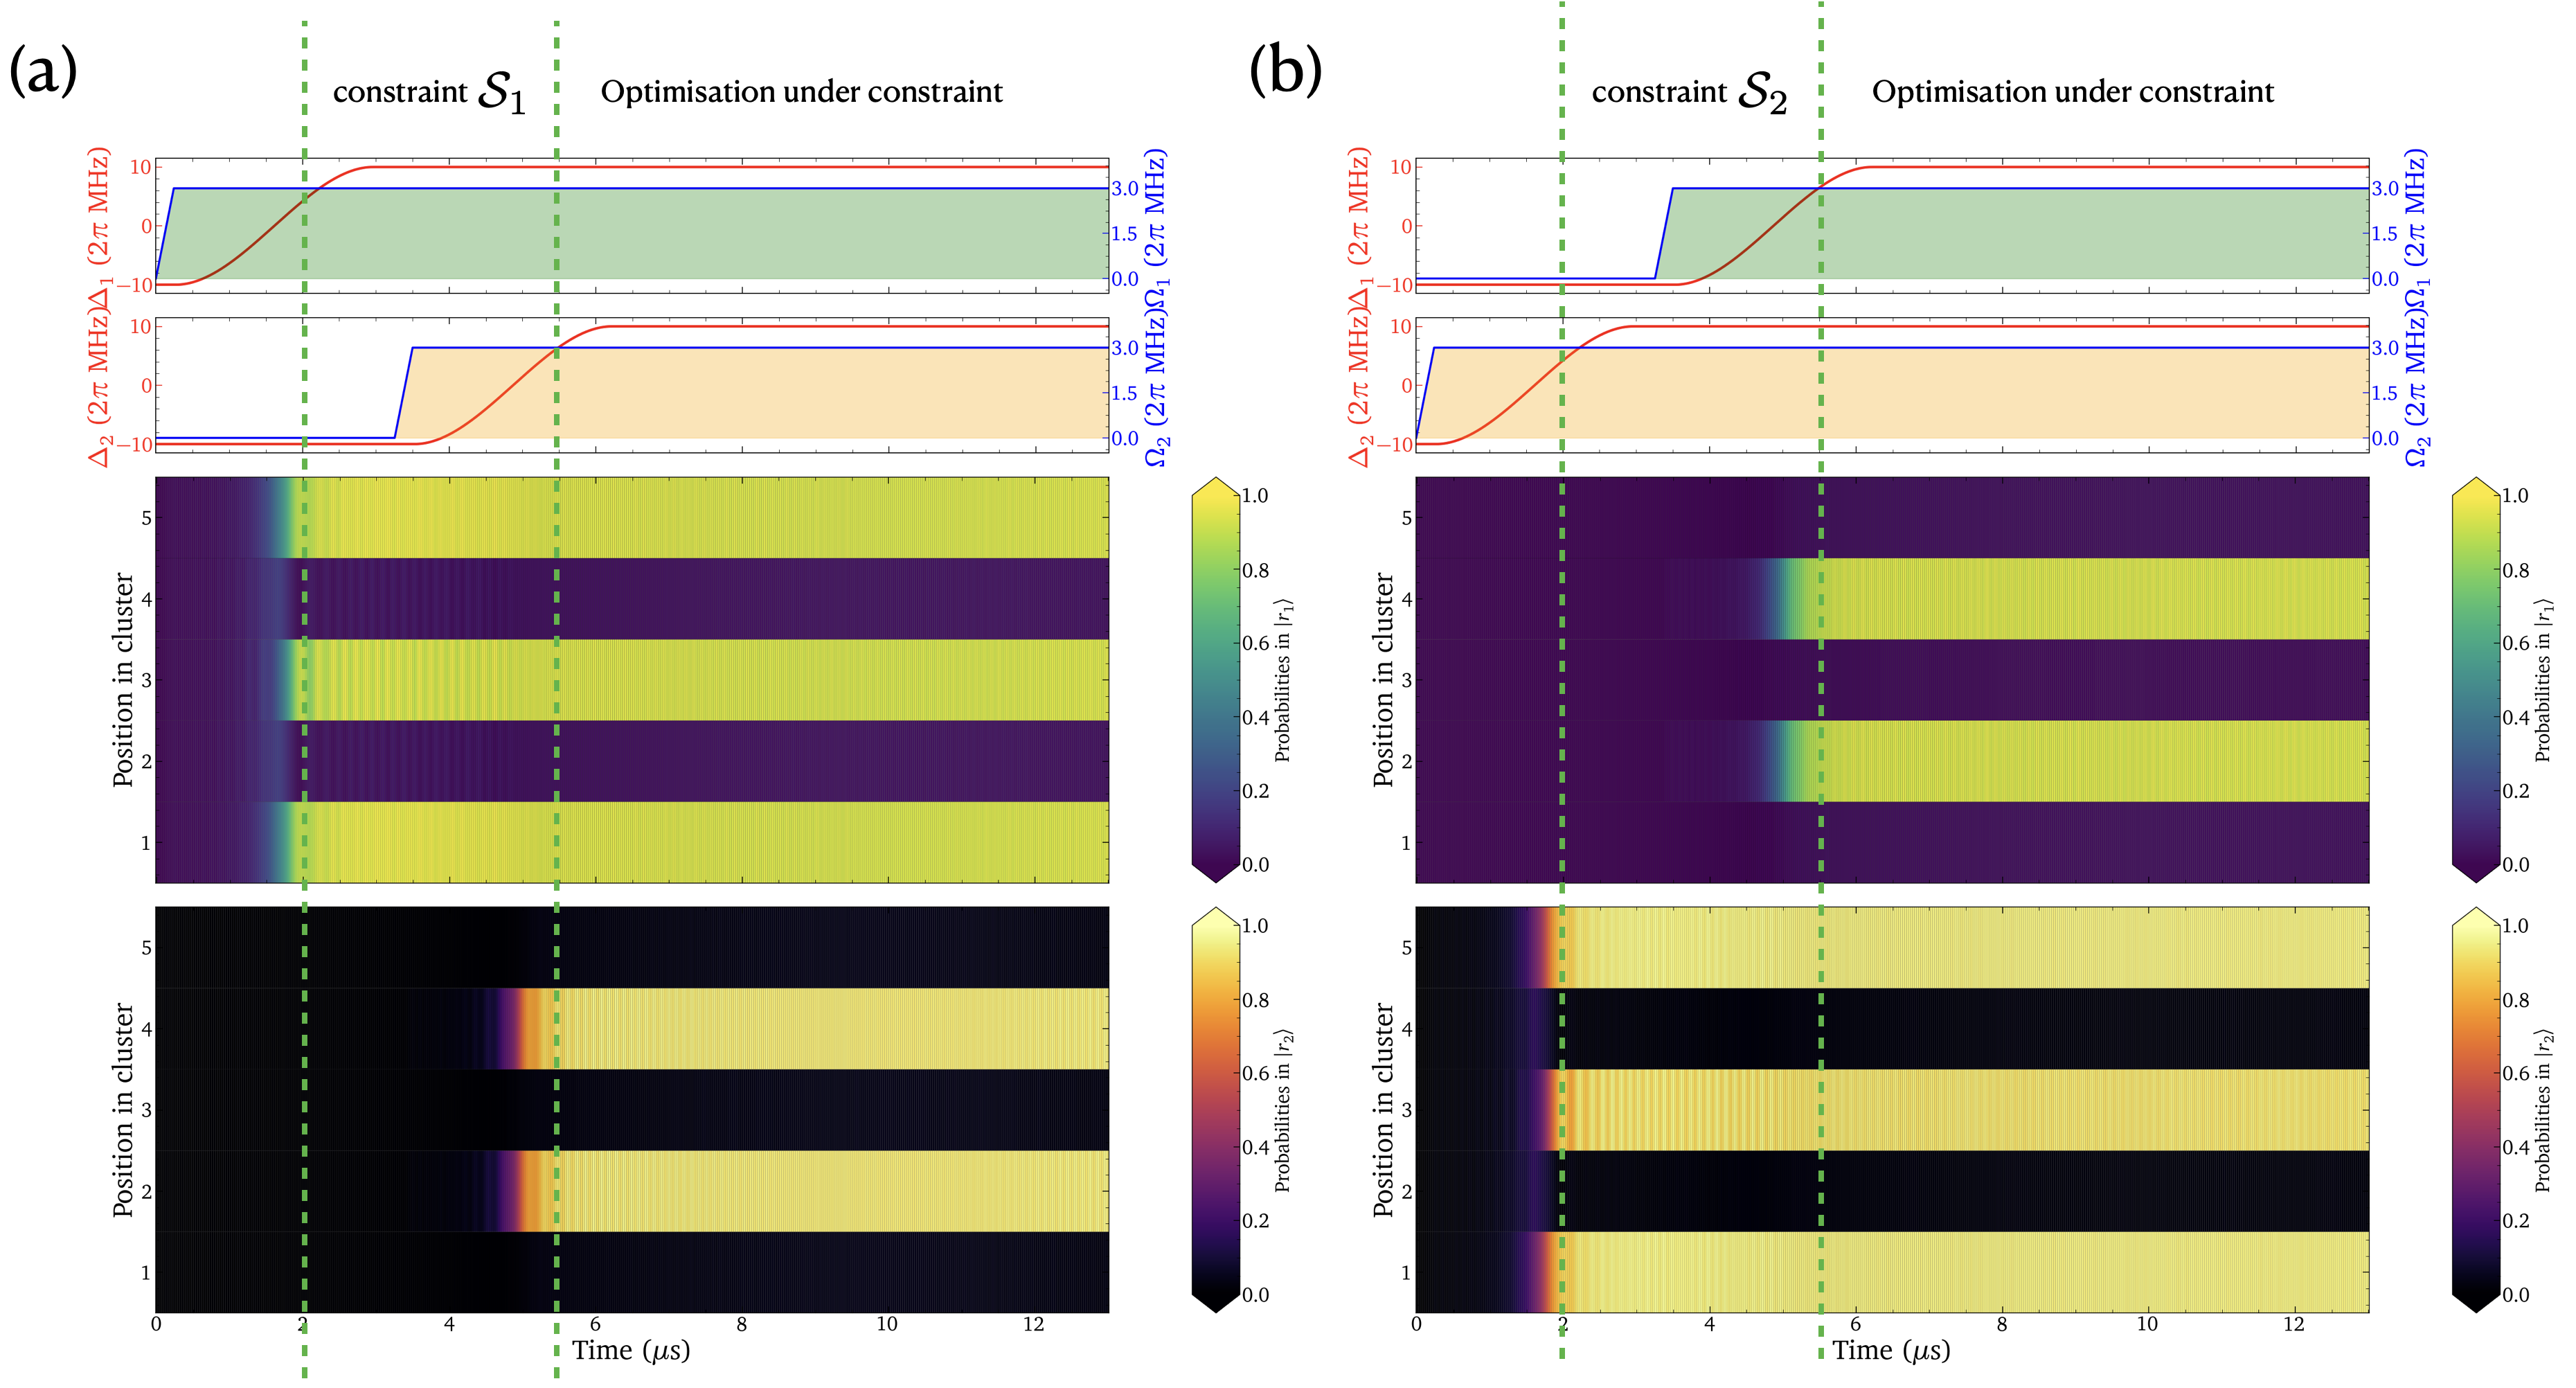
\includegraphics[width=14cm]{picture/case1_QOconstraint2.png}
    \caption{\textbf{$R^{(1)}_b:R^{(2)}_b:R^{(12)}_b=1:1:0.5$, and $a = 0.8R^{(1)}_b$}. The first graph of each figure shows the time-varying detunings $\Delta_1(t)$, $\Delta_2(t)$ (being swept in order), and Rabi frequencies $\Omega_1(t)$ (green shaded area), and $\Omega_2(t)$ (orange shaded area), the second graph shows the fidelity in the Rydberg state $\ket{r_1}$ denoted by green vertex, and the third graph shows the fidelity in the Rydberg state $\ket{r_2}$ denoted by orange vertex. The first sweeping is to encode associated constraints into the annealing state, called "constrained states". The second sweeping is to anneal the constrained states to a solution state in which the cost function is minimized under the constraint imposed by the first sweeping. (a) Optimization with constraint that the solution is lied in the $\mathcal{S}_1$ region. (b) Optimization with constraint that the solution is lied in the $\mathcal{S}_2$ region.}
    \label{fig:case1_sequential_driving_1}
\end{figure*}
On the other hand, the results from Fig.\ref{fig:case1_sequential_driving_2} correspond to the graph structure in Fig.\ref{fig:graph_mapping}(b), which yield the solutions to Max-3CM as the matching (all edges labelled by thick black color) is maximized under the given 3 colors (green, orange, blue), yet the matching is not perfect as the edge $(2,4)$ is not included due to the same color of the adjacent vertices (atom 2 and 4). Here, we say that the problems encoded into this kind of graph structure (Fig.\ref{fig:graph_mapping}(b)) need at least 4 colors to perfect the matching, and to become the solution to GCP problem. 

\subsection{$R^{(1)}_b:R^{(2)}_b:R^{(12)}_b=1:2:0.5$, {\rm and} $a=0.8R^{(1)}_b$.} 
From the scales of interaction strengths and the size of lattice spacings, the interaction between atoms in $\ket{r_1}$ is weaker than the interaction between atoms in $\ket{r_2}$, and since the blockade radius $R^{(1)}_b$ is covered the nearest neighboring atoms that make the atom array arrange themselves to be in $\mathbb{Z}_2$ order if they are all excited to $\ket{r_1}$ and to be in $\mathbb{Z}_3$ order if they are all excited to $\ket{r_2}$. Here, we define 2 low energy subspaces 
\begin{align}\label{subspace_case1}
     & \mathcal{S}_1 = \{ \ket{\psi} \hspace{1mm} :\hspace{1mm} n^{(i)}_1 n^{(i+1)}_1 \ket{\psi} = 0  \} \nonumber \\
     & \mathcal{S}_2 = \{ \ket{\psi} \hspace{1mm} :\hspace{1mm} n^{(i)}_2 n^{(i+d)}_2 \ket{\psi} = 0 \hspace{3mm} \textit{\rm for any} \hspace{3mm} d \leq 2 \}
\end{align}

This means that it is impossible to find two nearest atoms being excited in $\ket{r_1}$ in subspace $\mathcal{S}_1$, and is also impossible to find two nearest or next nearest atoms being excited in $\ket{r_2}$ in subspace $\mathcal{S}_2$. This can be seen in Fig.\ref{fig:case23_ground_barplot}(a), where we calculate the configuration of Rydberg excitations of atom array in the ground and excited states (Details of calculation are attached in the caption). The ground state here actually lie in $\mathcal{S}_1$, and the first excited state lied in $\mathcal{S}_2$. Obviously, as the $R^{(2)}_b > R^{(1)}_b$, the energy of subspace $\mathcal{S}_2$ is greater than the energy of subspace $\mathcal{S}_1$, i.e., $\bra{\mathcal{S}_2}H_{\rm Ryd}\ket{\mathcal{S}_2} > \bra{\mathcal{S}_1}H_{\rm Ryd}\ket{\mathcal{S}_1}$. From adiabatic theorem, the annealing state is supposed to stay at the ground energy level of the instantaneous Hamiltonian $H_{\rm Ryd}(t)$ during an adiabatic evolution, which allow no chance for quantum states $\ket{\psi} \in \mathcal{S}_2$ to jump up during such an evolution. However, we have shown that, by using the sequential detuning sweeping protocols, one can drive annealing states into quantum states in slightly higher energy level as shown in Fig.\ref{fig:case2_opt}.




\section{Extended data}

\begin{figure}[ht!]
    \centering
    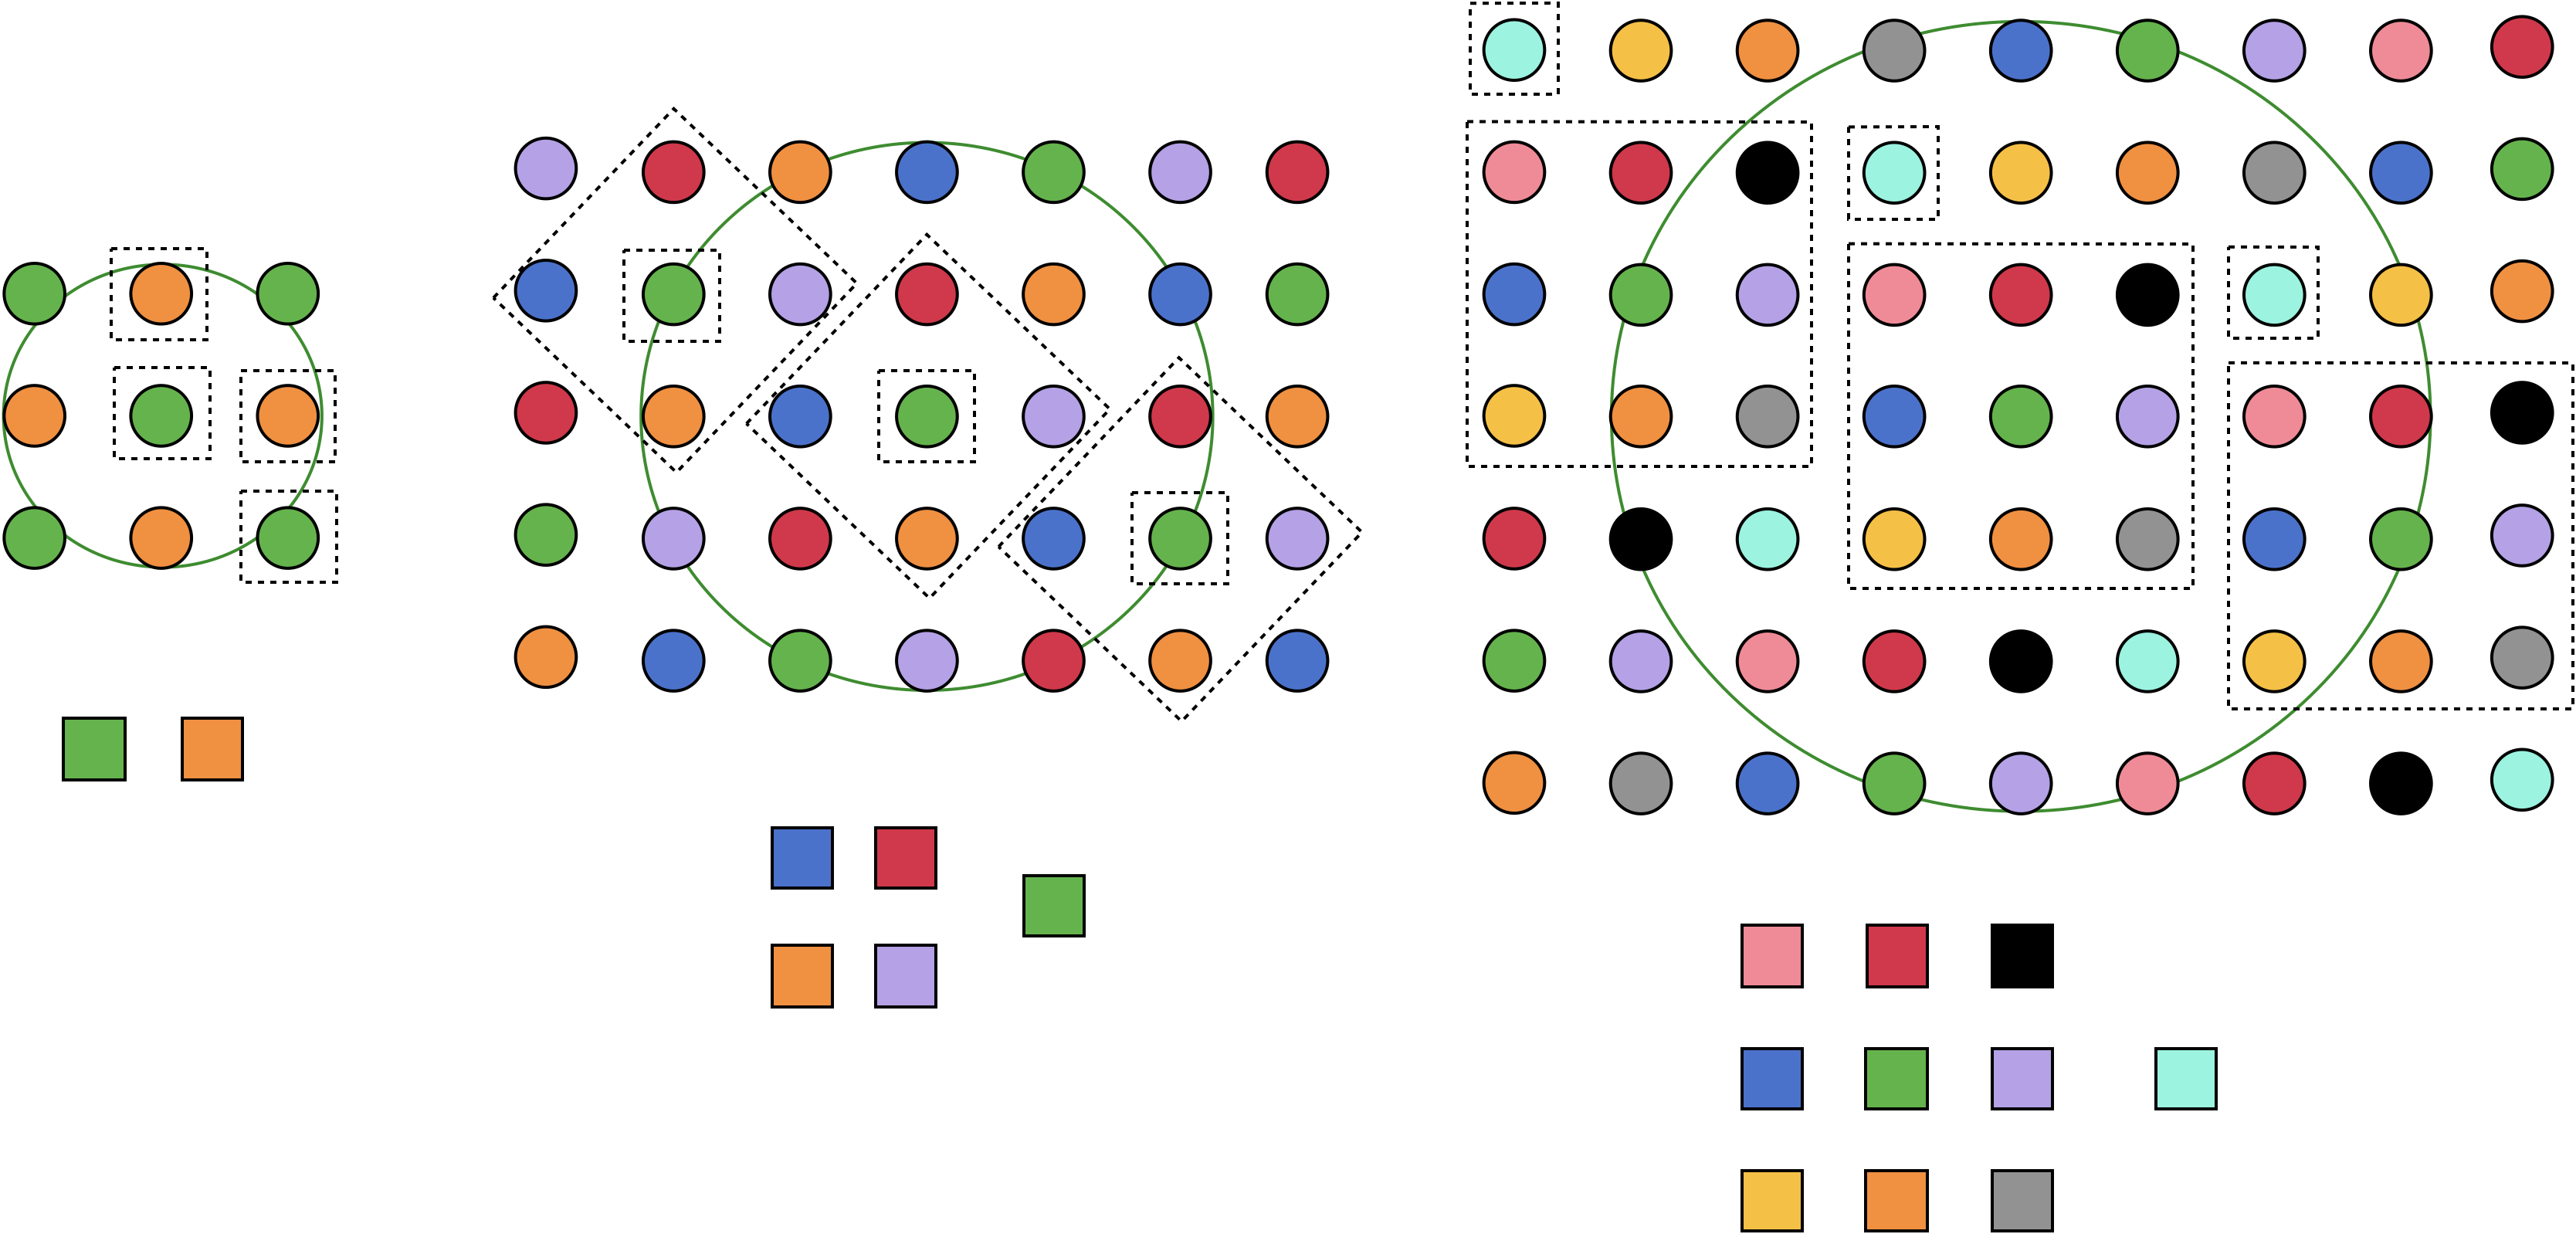
\includegraphics[width=15cm]{picture/2D_array_coloring.png}
    \caption{\textit{@D array chromatic number}}
    \label{fig:case2_opt}
\end{figure}


\begin{figure}[ht!]
    \centering
    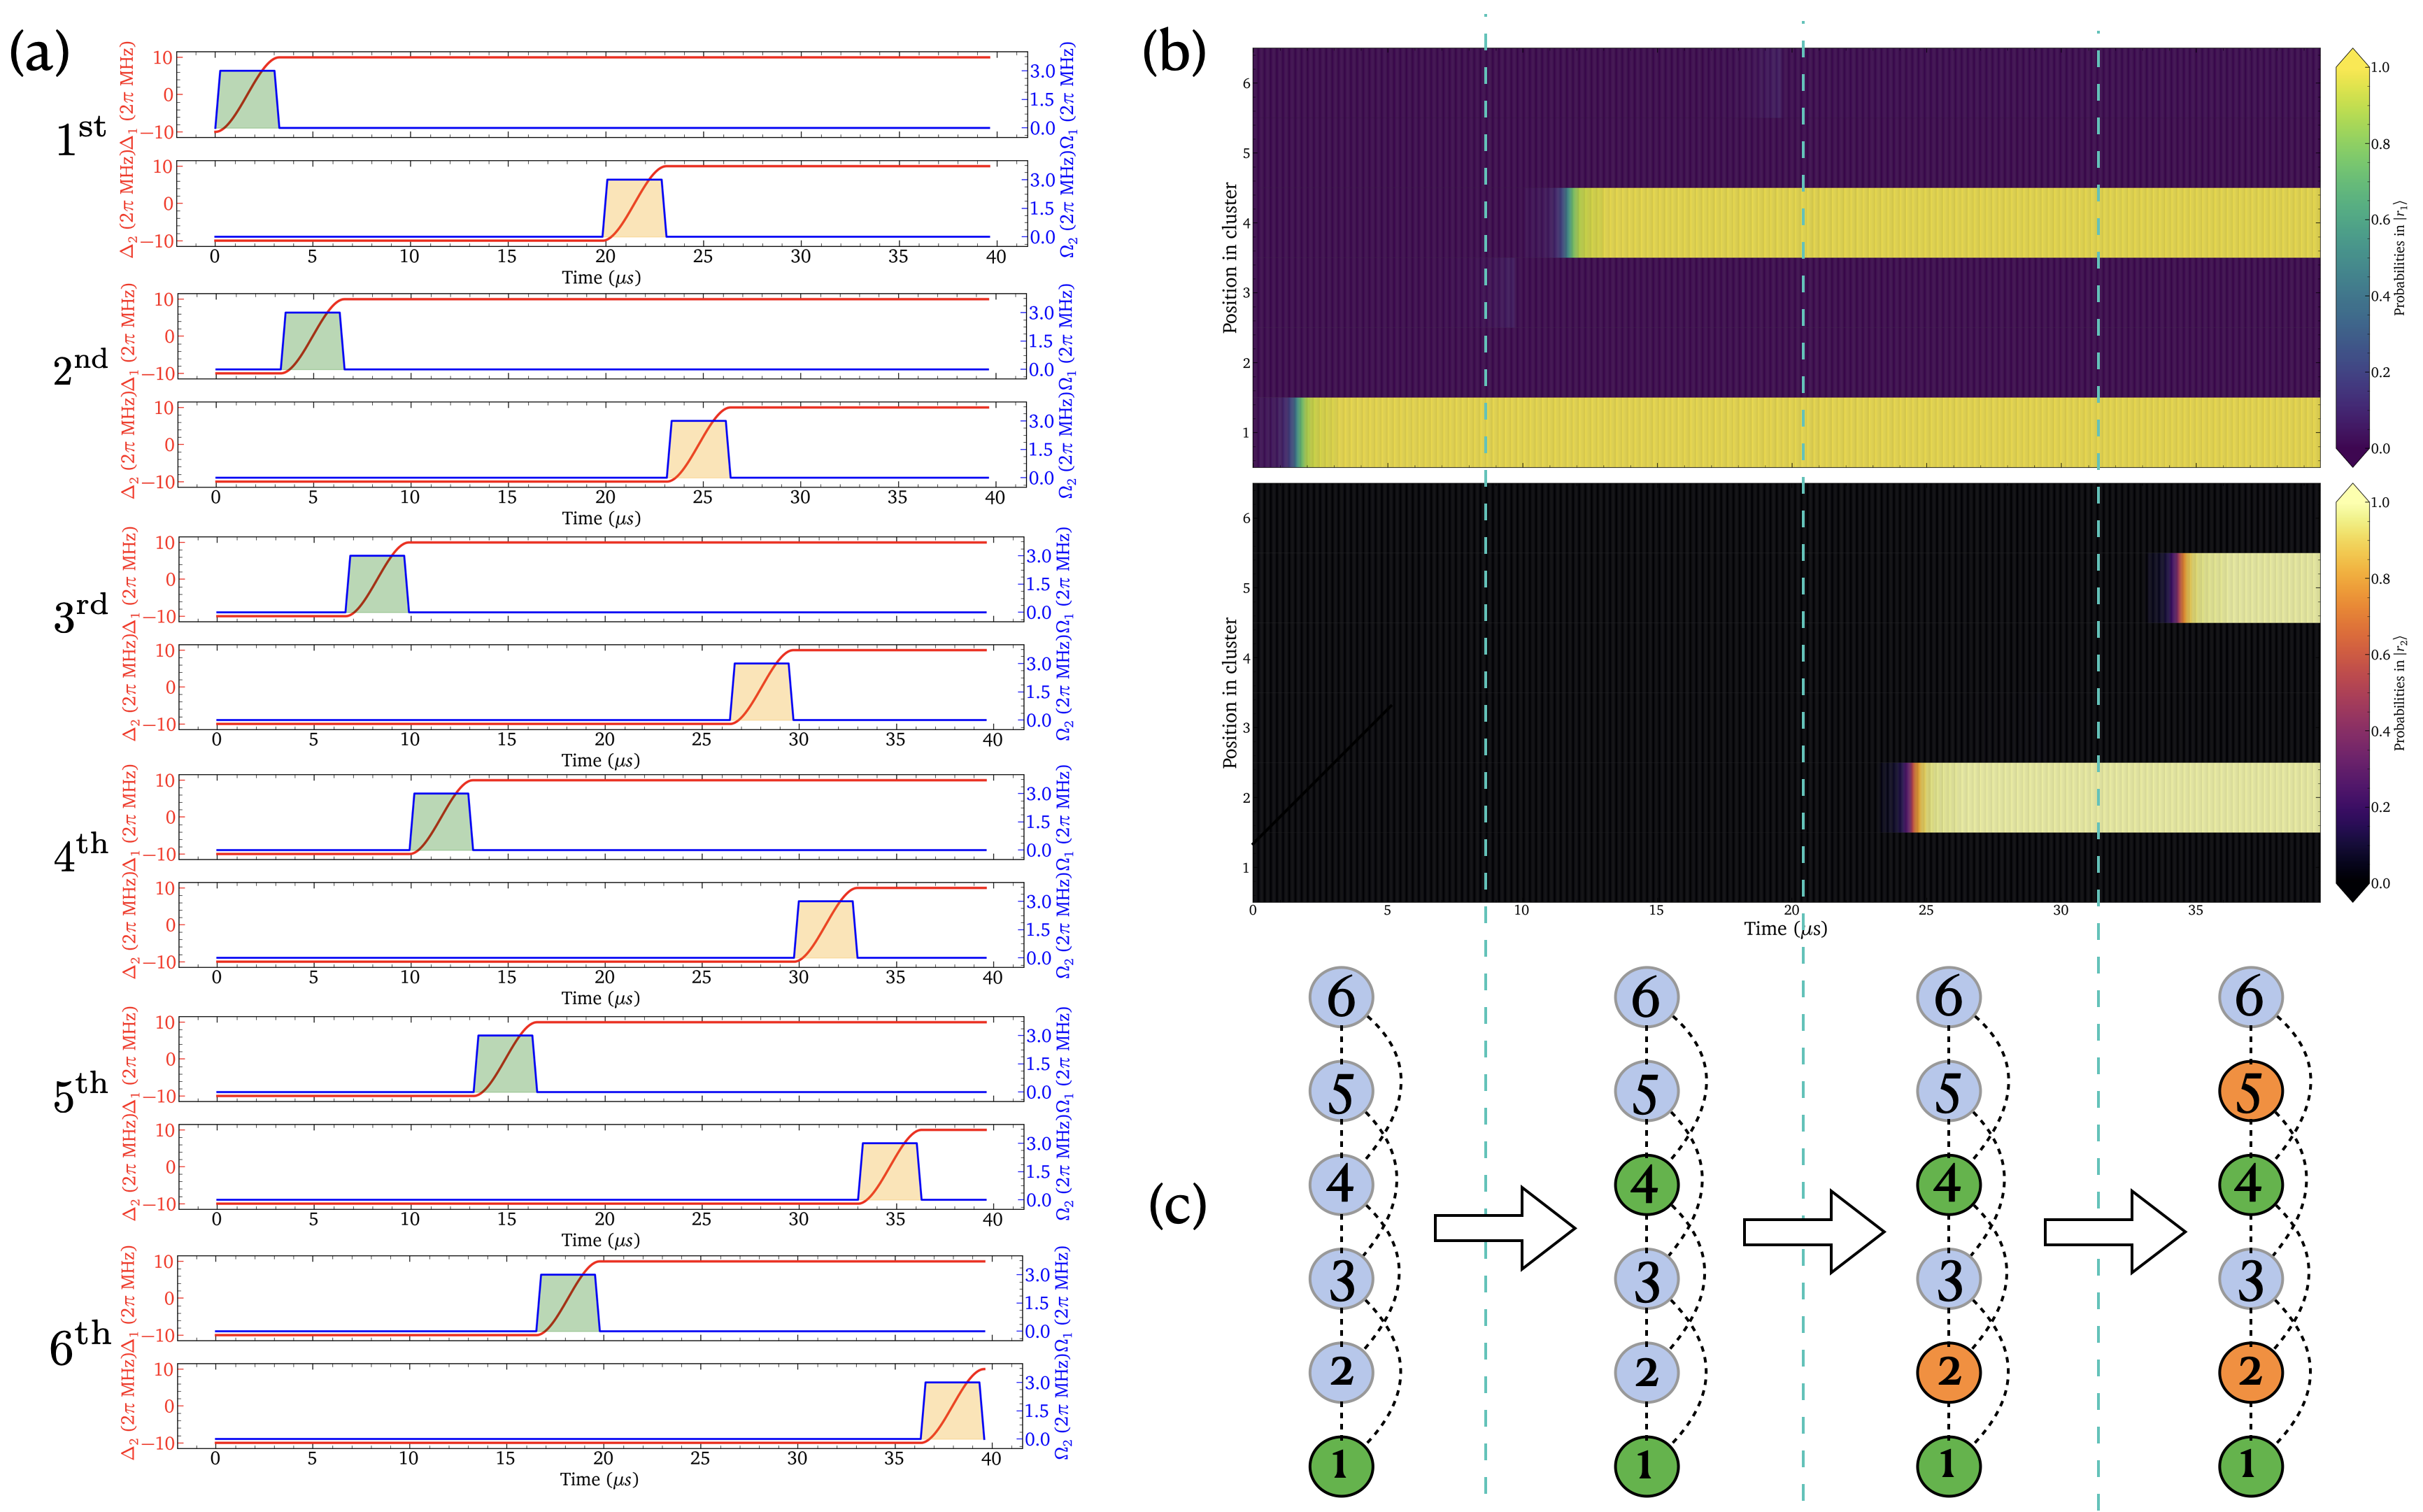
\includegraphics[width=14cm]{picture/GCP_6atom.png}
    \caption{\textit{Optimization with constraints}}
    \label{fig:case3_opt}
\end{figure}


\end{document}